\documentclass[12pt,a4paper, twoside]{article}
\usepackage[utf8]{inputenc}
\usepackage[italian]{babel}
\usepackage{graphicx}
\usepackage{subcaption}
\usepackage{float} % Opzionale, per un posizionamento più preciso
\usepackage{amsmath}
\usepackage{physics}
\graphicspath{{Immagini/}}
\usepackage{caption}

\usepackage[a4paper, % Margini 
top=2cm, 
bottom=2cm, 
left=2cm, 
right=2cm, 
bindingoffset=5mm]{geometry} %tesi stampata

\usepackage{fancyhdr}
\pagestyle{fancy}
\fancyhf{} % Pulisce tutti i campi correnti

% Linea in alto (Intestazione)
\renewcommand{\headrulewidth}{0.4pt} % Spessore linea superiore

% Linea in basso (Piè di pagina)
\renewcommand{\footrulewidth}{0.4pt} % Spessore linea inferiore

% Configurazione Footer (Numero pagina)
\fancyfoot[RO, LE]{\thepage}


\captionsetup[figure]{labelfont=bf, textfont=normalfont, labelseparator=colon}
\captionsetup[table]{labelfont=bf, textfont=normalfont, labelseparator=colon}
\usepackage[colorlinks=true, linkcolor=blue]{hyperref}
\usepackage[acronym, nonumberlist, automake]{glossaries} % Aggiunto automake
\makeglossaries
\setglossarystyle{list} % Oppure 'super' per un allineamento a colonna molto preciso
\newacronym{acs}{ACS}{Anti-Coincidence Scintillator}
\newacronym{cl}{CL}{GAGG scintillating calorimeter}
\newacronym{esa}{ESA}{European Space Agency}
\newacronym{fbk}{FBK}{Fondazione Bruno Kessler}
\newacronym{gagg}{GAGG}{Gadolinium Aluminum Gallium Garnet}
\newacronym{gbm}{GBM}{Gamma-ray Burst Monitors}
\newacronym{gbw}{GBW}{Gain Band-Width}
\newacronym{ldo}{LDO}{Low-Dropout Regulator}
\newacronym{leo}{LEO}{Low Earth Orbit}
\newacronym{opamp}{OPAMP}{Operational Amplifier}
\newacronym{pid}{PID}{Particle Identification}
\newacronym{sipm}{SiPM}{Silicon Photomultiplier}
\newacronym{sd}{SD}{Silicon Detector}
\newacronym{snr}{SNR}{Signal-to-Noise-Ratio}
\newacronym{spad}{SPAD}{Single Photon Avalanche Diodes}
\newacronym{tia}{TIA}{Transimpedence Amplifier}

\usepackage{chngcntr}

% Reset dei contatori all'inizio di ogni sezione
\counterwithin*{figure}{section}
\counterwithin*{table}{section}

% Ridefinizione dello stile della numerazione: NumeroSezione.NumeroOggetto
\renewcommand{\thefigure}{\thesection.\arabic{figure}}
\renewcommand{\thetable}{\thesection.\arabic{table}}
\usepackage[strings]{underscore}

%Bibliografia
\usepackage[style=ieee, backend=biber]{biblatex} % Carica il pacchetto con stile IEEE
\addbibresource{biblio.bib} % Specifica il file del database (con estensione .bib)

\begin{document}
	
	\begin{titlepage}
		\begin{center}
			% LOGO CON INTESTAZIONE INTEGRATA
			\vspace*{-1cm} % Tira leggermente su l'immagine se necessario
			
\includegraphics[width=0.5\textwidth]{unitn.png}\\[3.5cm] 
			
			% TIPO DI ELABORATO E TITOLO
			{\Large Elaborato di Laurea Triennale}\\[1.5cm]
			{\Huge \textbf{Sistemi di Condizionamento e Lettura\\[0.3cm] per Sensori SiPM nel Progetto SPaRKLE}}\\[3.5cm]
		\end{center}
		
		% BLOCCO RELATORE E LAUREANDO AFFIANCATI (Intatto)
		\begin{minipage}[t]{0.45\textwidth}
			\begin{flushleft}
				\large
				\textit{Relatore:}\\
				\textbf{Prof. Lucio Pancheri}\\[0.6cm]
				\textit{Correlatore:}\\
				\textbf{Matteo Polo}
			\end{flushleft}
		\end{minipage}
		\hfill
		\begin{minipage}[t]{0.45\textwidth}
			\begin{flushright}
				\large
				\textit{Laureando:}\\
				\textbf{Matteo Lonardi}\\
				Mat. 244095
			\end{flushright}
		\end{minipage}
		
		% SPINGE L'ANNO ACCADEMICO SUL FONDO DEL FOGLIO
		\vfill 
		
		\begin{center}
			\large Anno Accademico 2025/2026
		\end{center}
	\end{titlepage}
	
	% \tableofcontents
	% \clearpage
	\mbox{}
	\newpage
	\mbox{}
	\vspace{6cm}
	\begin{flushright}
		frase d'effetto
	\end{flushright}
	\newpage
	\mbox{}
	
	\newpage
	\tableofcontents
	
	\newpage
	\mbox{}
	
	\cleardoublepage
	\listoffigures
	
	\cleardoublepage
	\listoftables
	\newpage
	
	\cleardoublepage
	
	\printglossary[type=\acronymtype, title={Lista degli Acronimi}]
	
	\newpage
	
	\glsresetall % Reset Acronimi
	\section*{Abstract}
	\addcontentsline{toc}{section}{Abstract}
	
	Questo lavoro si basa sulla continuazione dello sviluppo di circuiti elettronici e condizionamento sulla base del lavoro svolto da Damiano Tessaro nell'a.a. 2024/2025. 
	\newpage
	\section{Introduzione} 
	\subsection{Space Rider e SPaRKLE}
	\begin{figure}[H]
		
\includegraphics[width=0.2\textwidth]{Immagini/spaceriderlogo}
		\label{fig:spaceriderlogo}
	\end{figure}
	
	
	Lo \textit{Space Rider} rappresenta il laboratorio orbitale riutilizzabile dell'Agenzia Spaziale Europea (ESA) progettato per garantire un accesso autonomo e versatile alla microgravità in orbita bassa (LEO).\\ Integrato sul vettore Vega-C, il sistema è in grado di ospitare fino a 600 kg di carico utile in un volume di 1.200 litri, fornendo supporto logistico, energetico e termico per missioni della durata di circa due mesi. Grazie alla capacità di rientro atmosferico e recupero del \textit{payload}, la piattaforma funge da ponte strategico tra la ricerca accademica, promossa tramite l'ESA Academy, e le applicazioni industriali nei settori farmaceutico e biomedico, semplificando l'operatività spaziale per attori non specialistici.
	\begin{figure}[H]
		\centering
		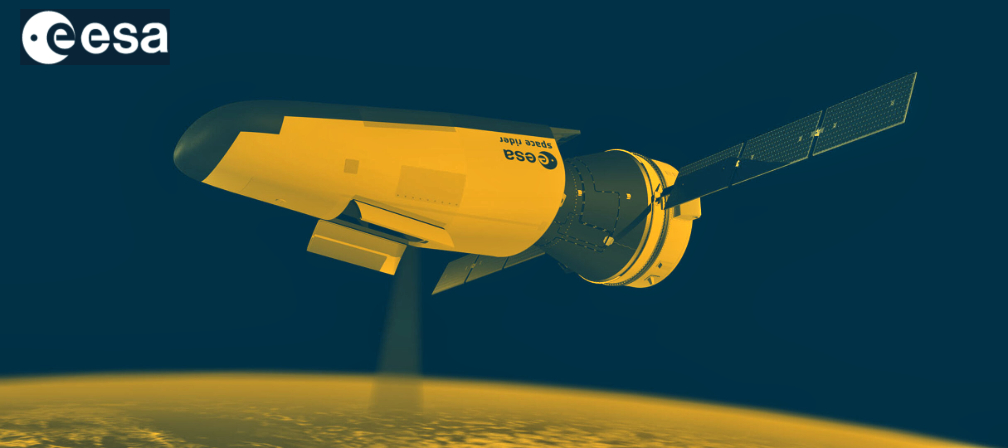
\includegraphics[width=0.8\textwidth]{Immagini/spacerider}
		\caption{Lo Space Rider nella LEO \cite{satnews_terran_2023}}
		\label{fig:spacerider}
	\end{figure}
	\newpage
	\begin{figure}[H]
		
\includegraphics[width=0.2\textwidth]{sparklelogo}
		\label{fig:sparklelogo}
	\end{figure}
	Il progetto \textit{Small Particle Recognition Kit for Low Energies} (SPaRKLE), sviluppato dall'Università di Trento e selezionato dall'ESA Academy, consiste in un laboratorio miniaturizzato per la rilevazione di radiazioni ionizzanti e particelle cariche in orbita bassa (\gls{leo}). Con un volume compatto di circa 1 dm$^3$ (equivalente a 1U CubeSat), il sistema è classificato come \textit{standard fixed payload} e richiede l'esposizione diretta all'ambiente spaziale per il monitoraggio di raggi X, raggi gamma e particelle a bassi livelli energetici.
	
	
	
	L'obiettivo primario della missione, oltre alla raccolta di dati astrofisici durante i due mesi di permanenza in orbita, è la validazione tecnologica dei fotomoltiplicatori al silicio (\gls{sipm}). Grazie alla capacità di recupero dello \textit{Space Rider}, SPaRKLE funge da dimostratore tecnologico, permettendo la caratterizzazione post-volo dei sensori e aprendo la strada all'impiego di strumentazione scientifica ad alta densità in future costellazioni di piccoli satelliti.
	
	\begin{figure}[H]
		\centering
		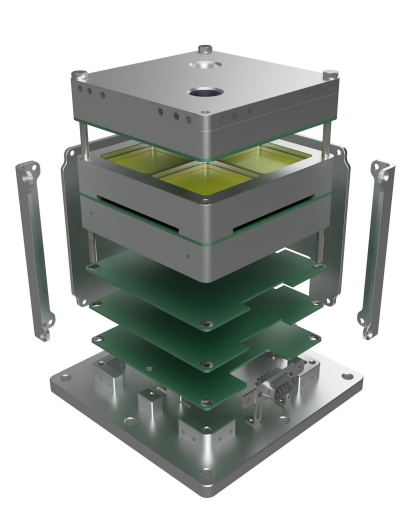
\includegraphics[width=0.5\textwidth]{sparklecube}
		\caption{una render esploso di SPaRKLE}
		\label{fig:sparklecube}
	\end{figure}
	\newpage
	\subsection{Sensori e Circuiti di Condizionamento}
	La rilevazione particellare nel dispositivo SPaRKLE si basa sulla distinzione tra interazioni continue e stocastiche. 
	
	Le \textbf{particelle cariche} (ioni ed elettroni) interagiscono mediante forze coulombiane, generando una ionizzazione lungo la traiettoria con deposizione energetica incrementale. 
	
	Diversamente, le \textbf{particelle neutre} (fotoni e neutroni) richiedono un singolo evento d'urto come l'effetto fotoelettrico o lo scattering Compton per trasferire energia a vettori carichi secondari; in assenza di tale interazione, esse possono attraversare il volume sensibile senza produrre segnali rilevabili.
	
	Il sistema all'interno di SPaRKLE utilizza la tecnica \textbf{$\Delta$E-E}, ovvero si vuole misurare la differenza di energia al passaggio di una particella per poi intrappolarla e misurarne l'effetiva energia.
	
	Per il \textbf{$\Delta$E}, si utilizza un rilevatore di silicio (SD) che misura una porzione di energia rilasciata dalla particella al suo passaggio.
	
	Invece per la parte \textbf{E} si utilizza uno scintillatore GAGG(\gls{gagg}) che misura l'energia rimanente della particella che si blocca nello scintillatore
	\begin{figure}[H]
		\centering
		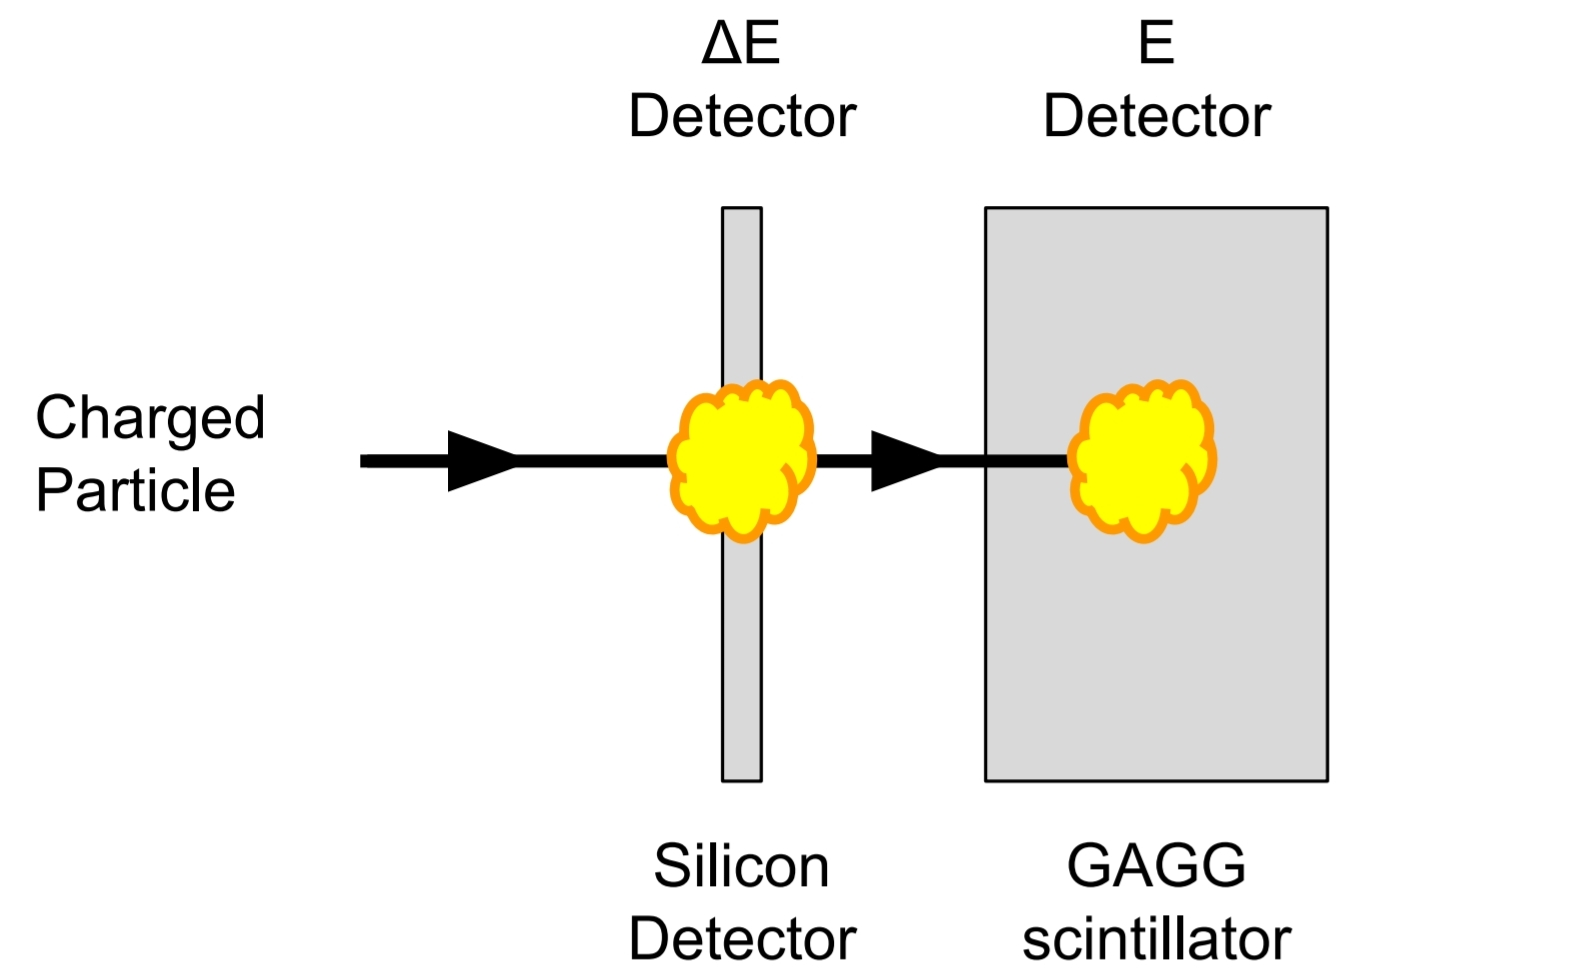
\includegraphics[width=0.9\textwidth]{deltaee}
		\caption{Rappresentazione schematica della tecnica $\Delta$E-E}
		\label{fig:deltaee}
	\end{figure}
	
	\newpage
	
	Per riconoscere il tipo di particella che attraversa SPaRKLE, bisogna distinguere i loro valori energetici.
	\begin{table}[H]
		\centering
		\begin{tabular}{l|r}
			\hline
			Tipo di particella & Energia \\ \hline
			Elettroni &  0.5-30 MeV \\ 
			Protoni &  5-90 MeV \\ 
			Fotoni & 0.01-30 MeV \\ \hline
		\end{tabular}
		\caption{{\small La tabella riporta i valori in MeV delle particelle rilevabili da SPaRKLE}}
	\end{table}
	
	\subsection{Panoramica del rilevatore}
	SPaRKLE contiene diversi moduli e sottomoduli per la rilevazione di particelle, racchiusi nel \textbf{Identificatore di Particelle} (\gls{pid}) in due blocchi PID_1 e PID_2
	\begin{itemize}
		\item Rilevatori al Silicio(\gls{sd}): SD_A1 e SD_A2 per la rilevazione delle particelle cariche
		\item Calorimetri scintillanti \gls{gagg} (\gls{cl}): CL_A1,CL_A2, CL_B1 e CL_B2. Sensibili a particelle cariche e fotoni (raggi-X e raggi-$\gamma$) che saranno letti dai fotomoltiplicatori al silicio (\gls{sipm}).
		\item Scintillatori anti-coincidenza(\gls{acs}): ACS_T(Top) e ACS_B (Bottom), utilizzati per la distinzione tra particelle cariche e fotoni data la somiglianza energetica.
		\item Monitor di lampi gamma (\gls{gbm}): GBM_1 e GBM_2 specializzati nella rilevazione di raggi-X e raggi-$\gamma$
	\end{itemize}
	\newpage
	\begin{figure}[!t]
		\centering
		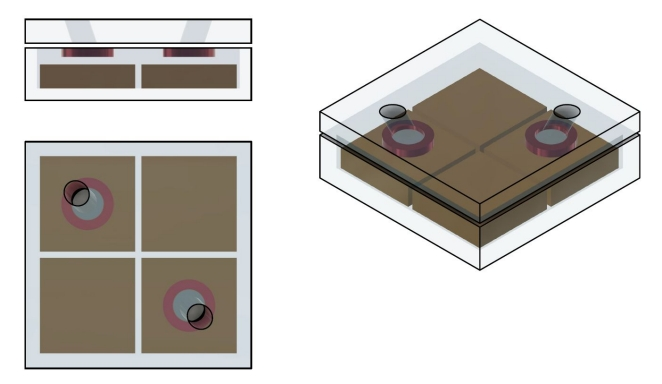
\includegraphics[width=0.75\textwidth]{detector1}
		\label{fig:detector1}
		\caption{Stilizzazione del blocco P/L di SPaRKLE}
	\end{figure}
	\begin{figure}[!t]
		\centering
		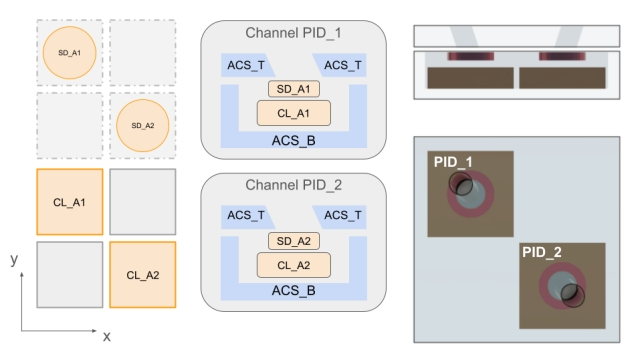
\includegraphics[width=0.75\textwidth]{detector2}
		\label{fig:detector2}
		\caption{Schematizzazione di PID_1 e PID_2 nella geometria P/L}
	\end{figure}
	\begin{figure}[H]
		\centering
		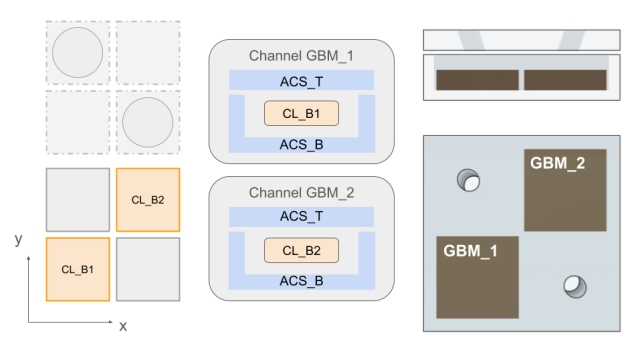
\includegraphics[width=0.75\textwidth]{detector3}
		\label{fig:detector3}
		\caption{Schematizzazione di GBM_1 e GBM_2 nella geometria P/L}
	\end{figure}
	
	\newpage
	
	\subsection{Fotomoltiplicatori al Silicio (\gls{sipm})}
	I \gls{sipm} sono molto sensibili a rilevare anche il singolo fotone. Sono composti da un'insieme di linee di diodi a valanga a singolo fotone (\gls{spad}) che operano in modalità Geiger, connessi in parallelo.
	\begin{figure}[H]
		\centering
		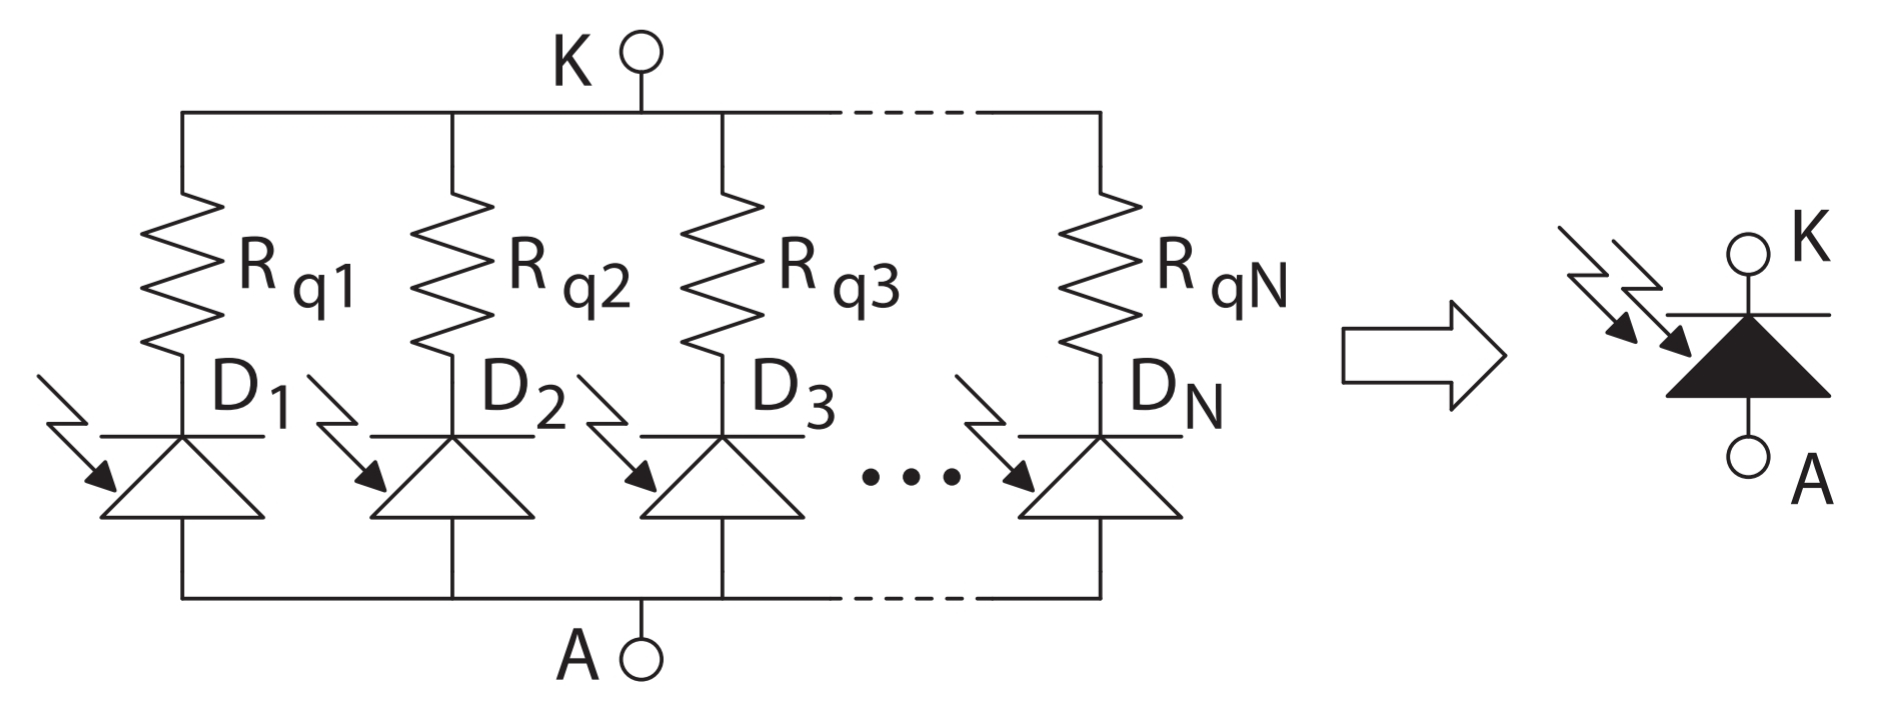
\includegraphics[width=0.7\textwidth]{spad}
		\label{fig:spad}
		\caption{Rappresentazione di N fotodiodi $D_i$ valanga  con le rispettive resistenze $R_i$ e connessi in parallelo}
	\end{figure}
	
	Tessaro Daminano sceglie un modello equivalente alle linee di diodi in Figura \ref{fig:spad}, dato il modello reale molto complesso, aumenta significativamente il tempo di simulazione. Il modello equivalente, più pratico è composto da un generatore di corrente, che simula l'impulso che il fotodiodo genererebbe quando un fotone innesca una scarica di Geiger 
	\begin{figure}[H]
		\centering
		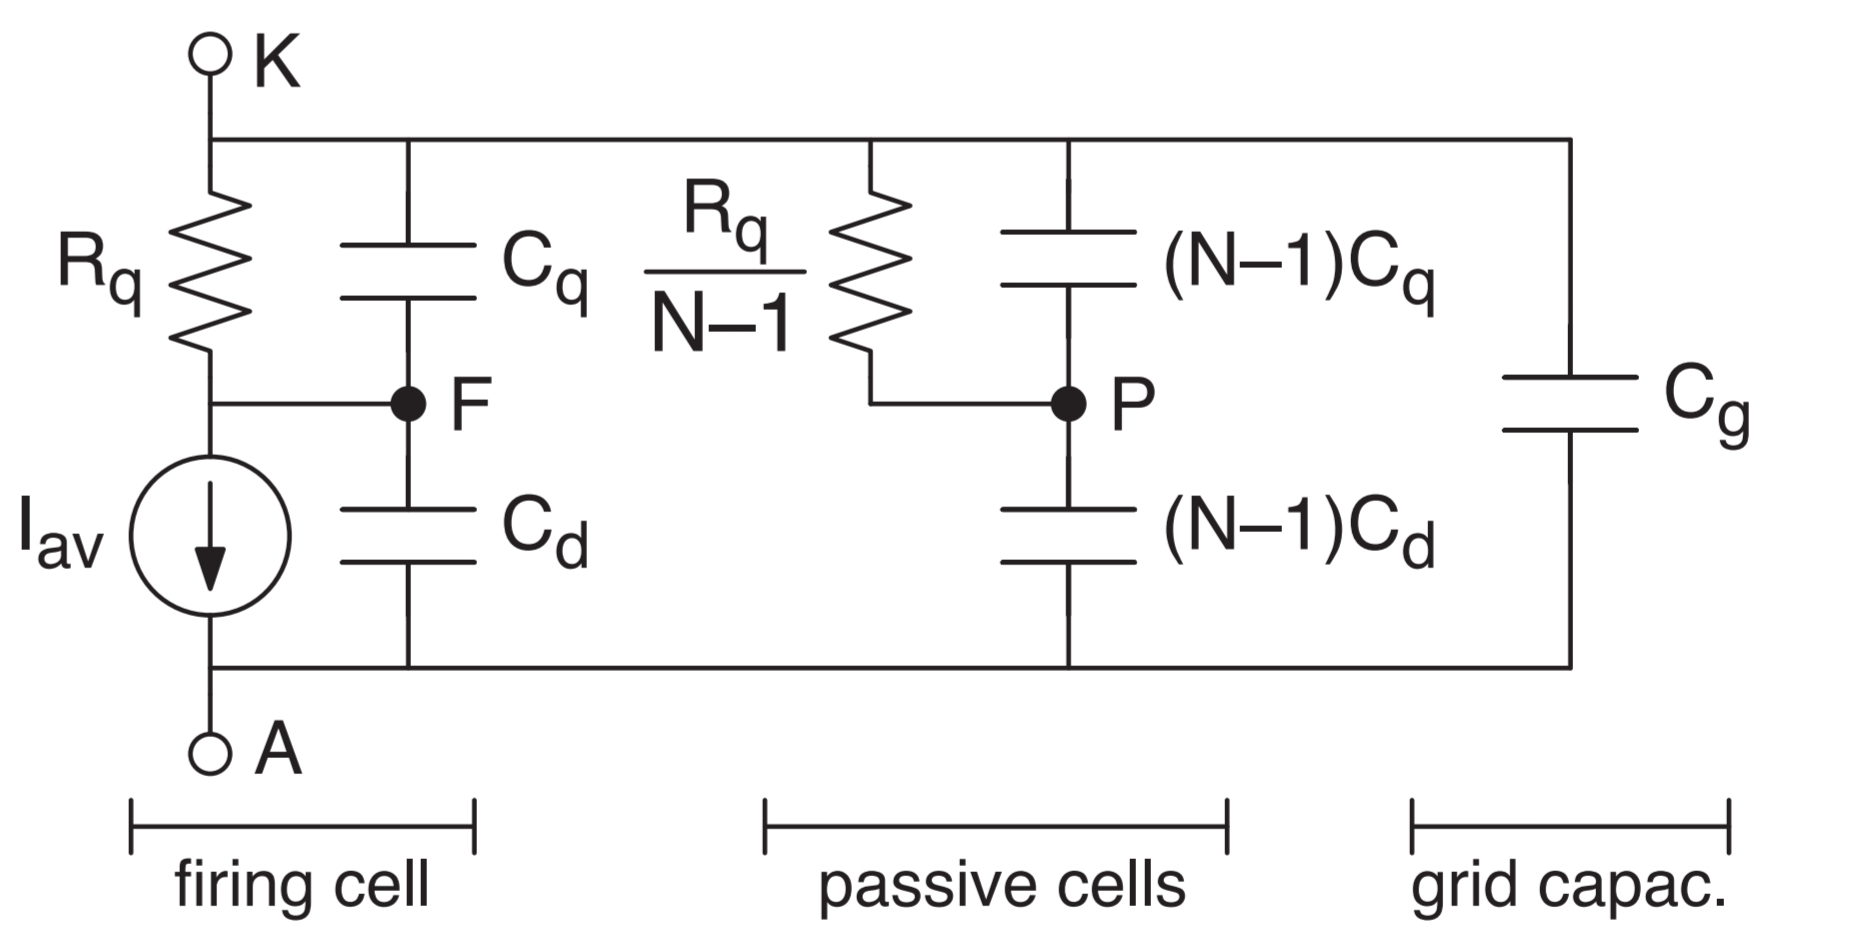
\includegraphics[width=0.7\textwidth]{spadeq}
		\caption{Modello di SPAD equivalente}
		\label{fig:spadeq}
	\end{figure}
	
	Nella realtà il sensore \gls{sipm} appare così, fornito da \gls{fbk}, dalla quale, con delle immagini al microscopio, possiamo estrapolare il numero di celle appartententi al sensore, così da avere un modello su LTspice più accurato possibile.
	
	\begin{figure}[H]
		\centering
		% Sottofigura di SINISTRA
		\begin{subfigure}[t]{0.48\textwidth} % Cambiato in [t]
			\centering
			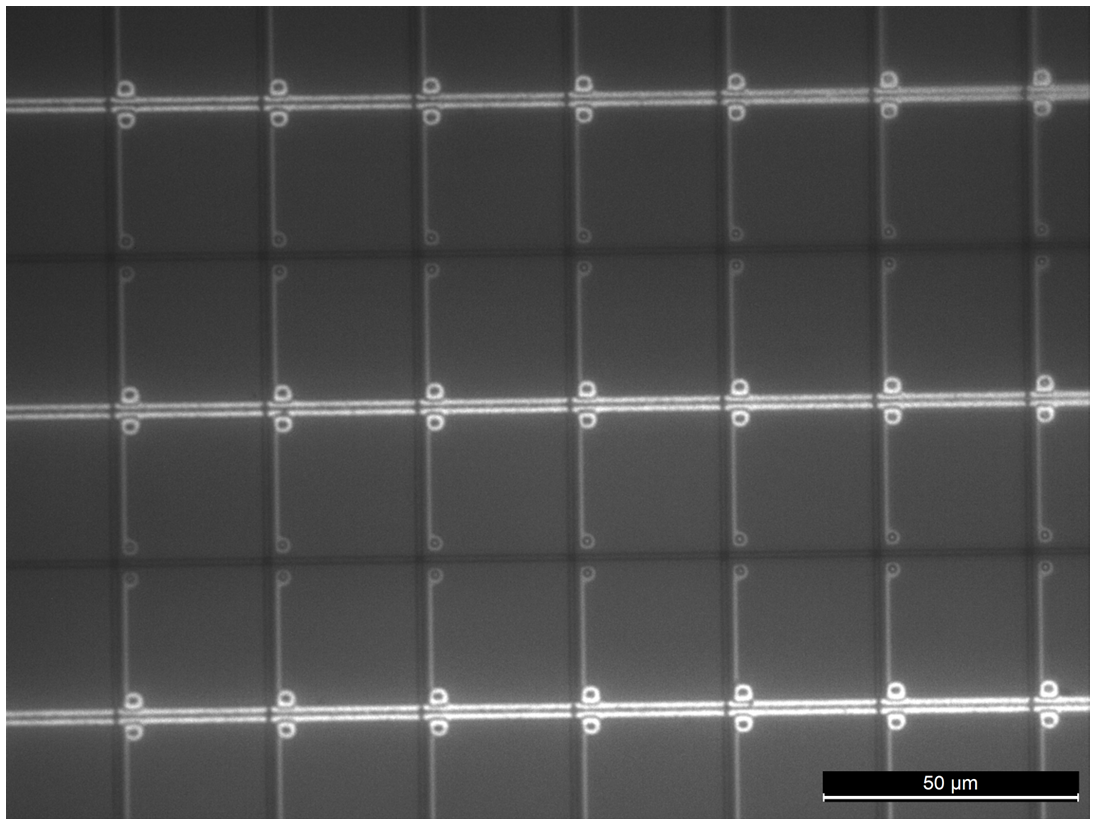
\includegraphics[width=\linewidth]{sipm50u}
			\caption{Immagine \gls{sipm} al microscopio con scala $50\mu m$.}
			\label{fig:sipm50u}
		\end{subfigure}
		\hfill
		% Sottofigura di DESTRA
		\begin{subfigure}[t]{0.48\textwidth} % Cambiato in [t]
			\centering
			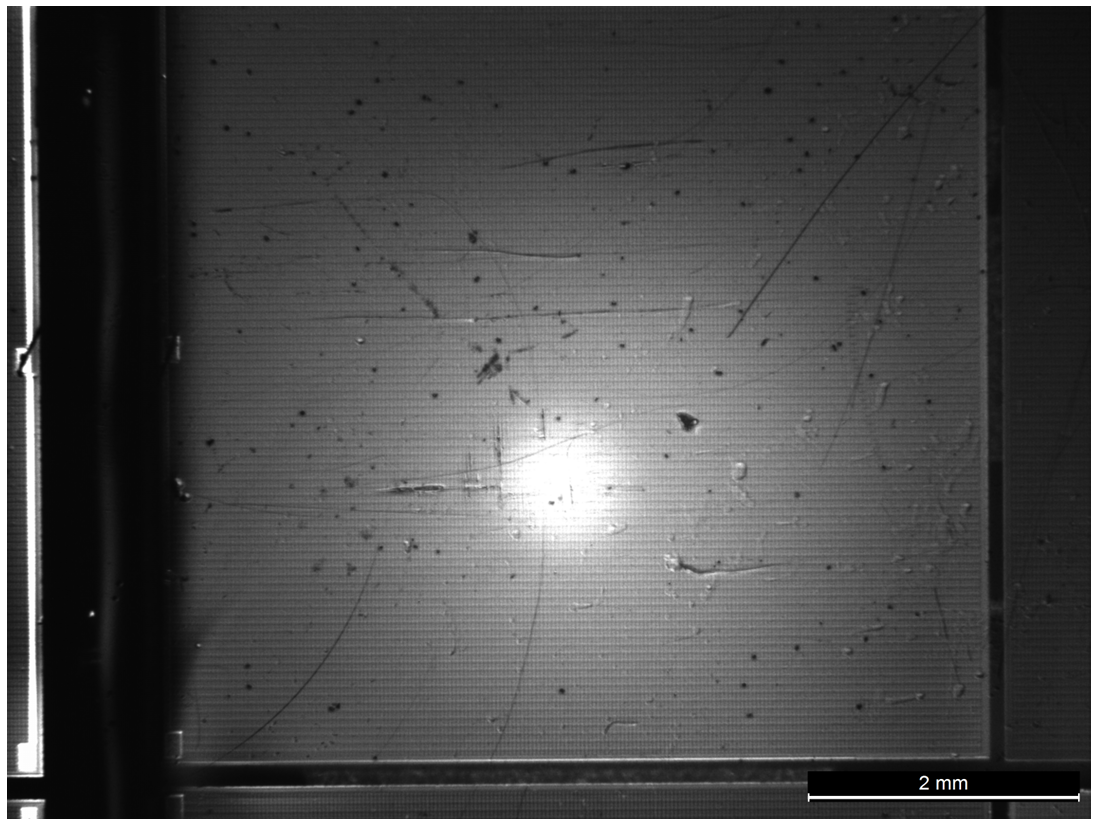
\includegraphics[width=\linewidth]{sipm2m}
			\caption{Immagine \gls{sipm} al microscopio con scala $2mm$.}
			\label{fig:sipm2m}
		\end{subfigure}
	\end{figure}
	
	Tessaro crea una database partendo da un singolo impulso , da cui genera trenta altri impulsi da diverse microcelle, ognuno scalato opportunamente per avere il riferimento del primo. A questo impulso viene effettuata una regressione a doppio esponenziale del tipo
	\begin{equation}
		\centering
		A1 e^{-\frac{t}{\tau 1}}+A2 e^{-\frac{t}{\tau 2}}
	\end{equation}
	
	\begin{figure}[H]
		\centering
		% Sottofigura di SINISTRA
		\begin{subfigure}[t]{0.48\textwidth} % Cambiato in [t]
			\centering
			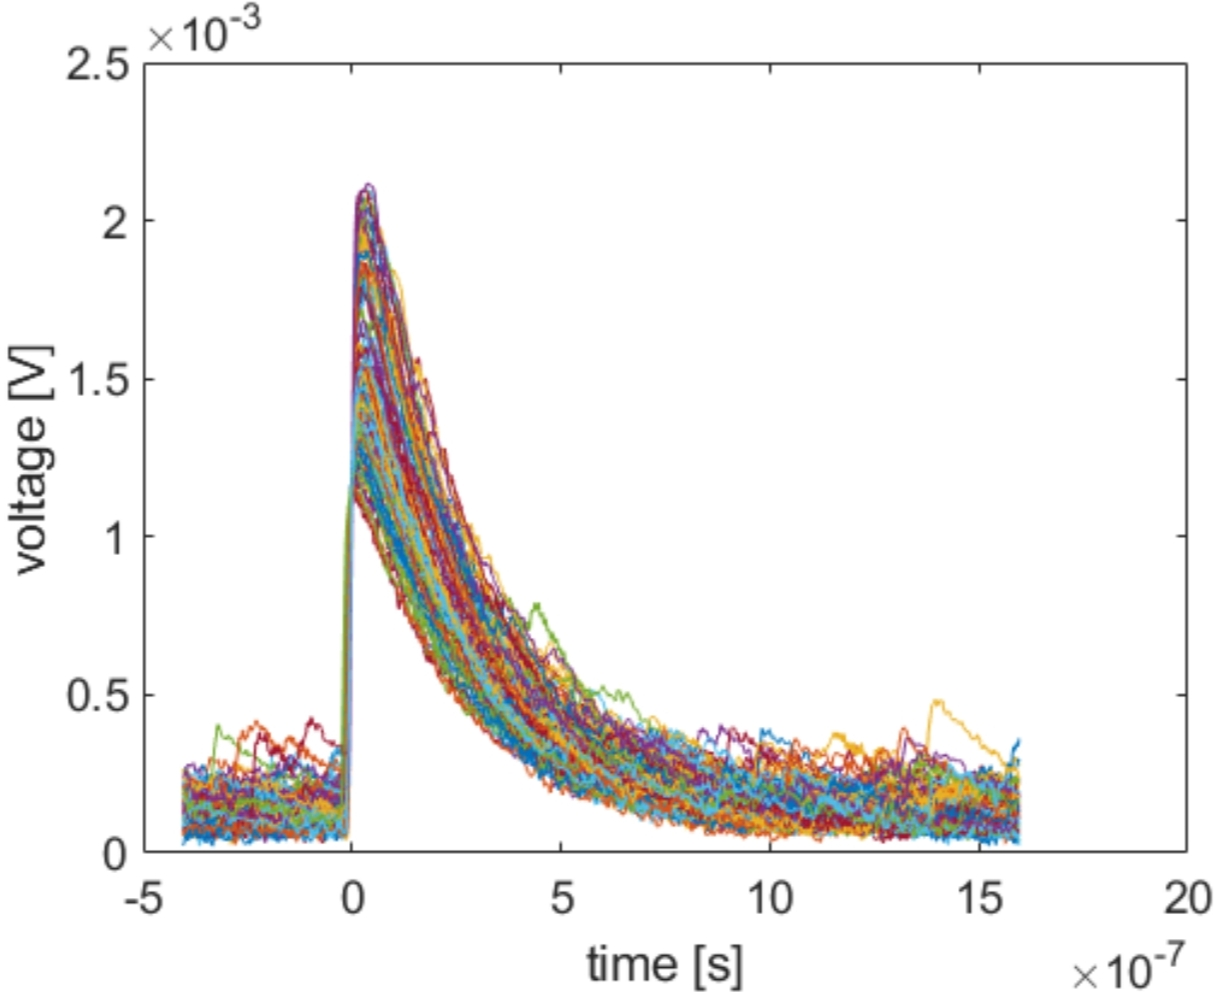
\includegraphics[width=\linewidth]{30imp}
			\caption{Venti forme d'onda di impulsi acquisiti da eventi multi-conteggio oscuro corrispondenti a 10-20 celle attive simultaneamente.}
			\label{fig:impulsi_multipli}
		\end{subfigure}
		\hfill
		% Sottofigura di DESTRA
		\begin{subfigure}[t]{0.48\textwidth} % Cambiato in [t]
			\centering
			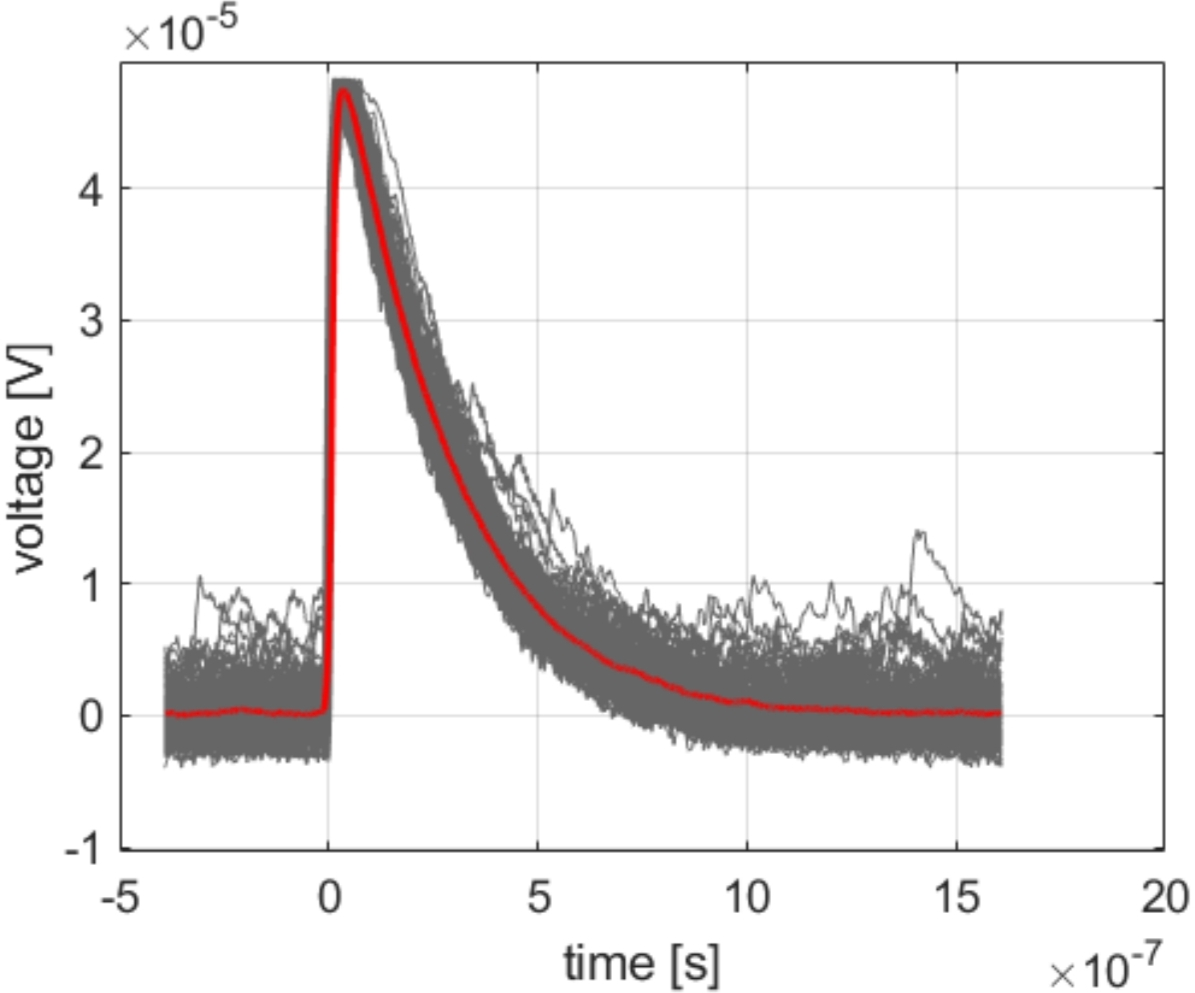
\includegraphics[width=\linewidth]{30impreg}
			\caption{Forme d'onda scalate per la medesima amplificazione di un singolo impulso (grigio). La curva rossa rappresenta la media sulla quale è stata eseguita la regressione.}
			\label{fig:regressione_impulsi}
		\end{subfigure}
		\caption{Analisi comparativa e regressione delle forme d'onda acquisite.}
	\end{figure}
	
	\begin{table}[H]
		\centering
		% Prima tabella (Sinistra)
		\begin{minipage}{0.48\textwidth}
			\centering
			\begin{tabular}{l|r}
				\hline
				Parametro & Valore \\ \hline
				$A_1$ & 2.917 $\mu V$ \\ 
				$A_2$ & 57.22 $\mu V$ \\ 
				$\tau_1$ & 471.3 $ns$ \\ 
				$\tau_2$ & 242.6 $ns$ \\ \hline
			\end{tabular}
			\caption{{\small Parametri della regressione a doppio esponenziale}}
		\end{minipage}
		\hfill % Spazio elastico centrale
		% Seconda tabella (Destra)
		\begin{minipage}{0.48\textwidth}
			\centering
			\begin{tabular}{l|r}
				\hline
				Parametro & Valore \\ \hline
				$R_q$ & 1.13 $M\Omega$ \\ 
				$C_q$ & 397 $fF$ \\ 
				$C_d$ & 18.1 $fF$ \\
				$C_g$ & 3.64 $nF$ \\
				$V_{br}$ & 27 $V$ \\ 
				$Q_{av}$ & 272.5 $fC$ \\ \hline
			\end{tabular}
			\caption{{\small Parametri elettrici del modello equivalente di \textbf{Figura} \ref{fig:spadeq}}}
		\end{minipage}
	\end{table}
	
	\begin{figure}[H]
		\centering
		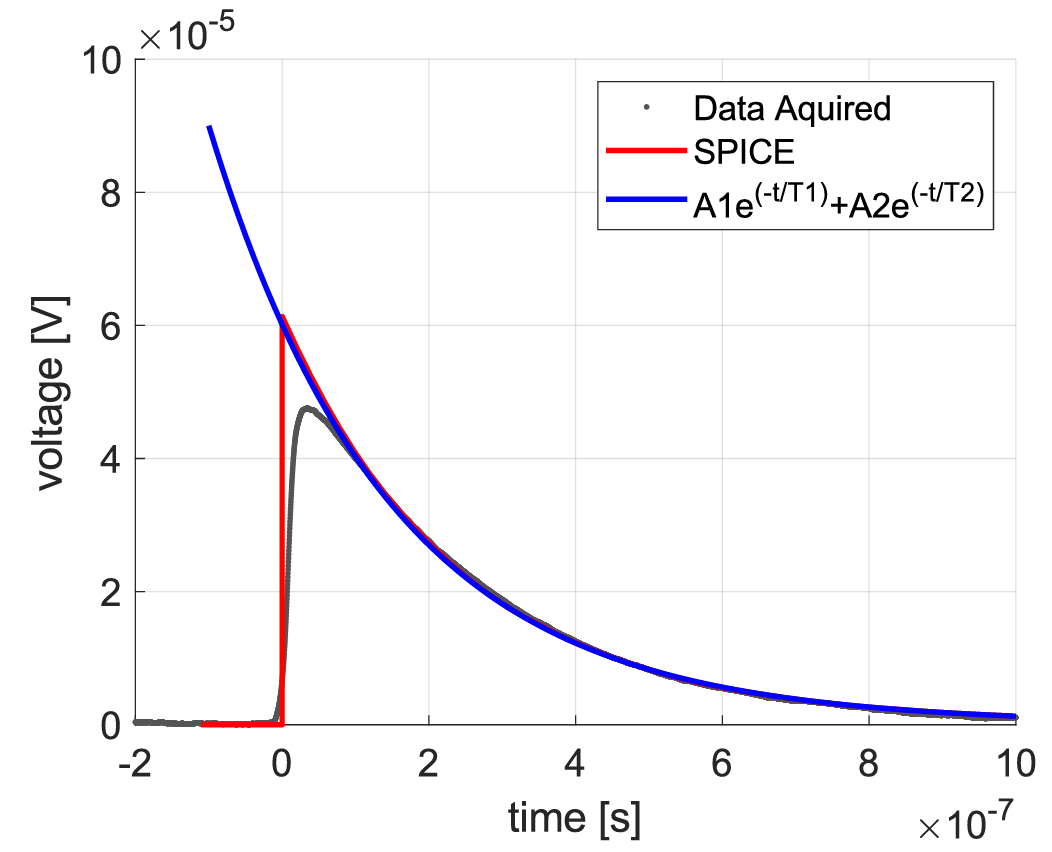
\includegraphics[width=0.7\textwidth]{reg}
		\label{fig:reg}
		\caption{Confronto tra dati acquisiti, il sensore simulato con LTspice e la regressione a doppio esponenziale}
	\end{figure}
	
	\section{Elettronica di lettura per \gls{sipm}}
	L'elaborazione dei segnali generati dai \gls{sipm} richiede un'elettronica dedicata capace di preservare l'accuratezza temporale e minimizzare il rumore. Si distinguono principalmente due approcci: il \textit{Voltage Mode} e il \textit{Current Mode}.
	
	\subsection{Voltage Mode}
	Per ottenere elevate prestazioni temporali, il preamplificatore deve garantire un tempo di salita rapido, rendendo necessaria un'ampia larghezza di banda. Quando si utilizza un amplificatore di tensione, la resistenza d'ingresso ($R_{IN}$) non può assumere valori elevati; di conseguenza, l'amplificatore deve fornire un guadagno sufficiente per garantire un'ampiezza del segnale di uscita adeguata alle elaborazioni successive, come l'integrazione per la misura dell'energia o la discriminazione per la misura del tempo.
	
	Tuttavia, l'approccio in tensione presenta alcune limitazioni critiche:
	\begin{itemize}
		\item \textbf{Consumo energetico:} ottenere un elevato prodotto guadagno-banda richiede un consumo di potenza significativo, risultando inefficiente per applicazioni con molti canali di lettura o bassi livelli di luce.
		\item \textbf{Degradazione del rumore:} il rumore di tensione equivalente in ingresso dell'amplificatore si somma direttamente alla tensione ai capi di $R_{IN}$, peggiorando il rapporto segnale-rumore (\gls{snr}) e limitando la risoluzione temporale.
	\end{itemize}
	
	
	A questo punto inizia il mio lavoro, ovvero la caratterizzazione e misure sulla scheda progettata da Damiano.
	
	\begin{figure}[H]
		\centering
		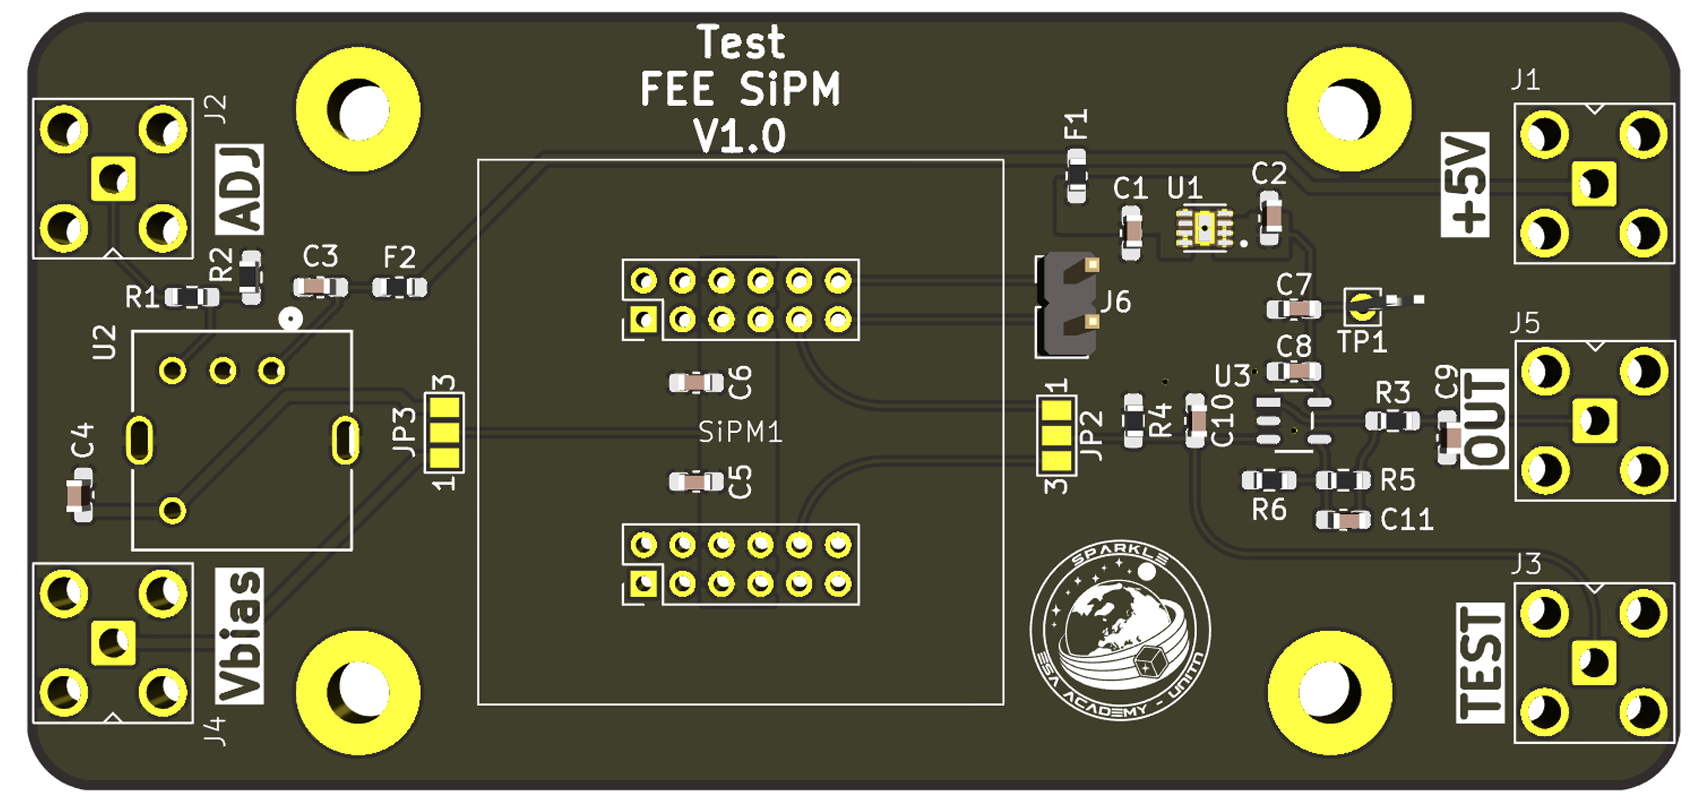
\includegraphics[width=0.7\textwidth]{scheda_voltagemode}
		\label{fig:scheda_voltagemode}
		\caption{Circuito stampato del controllo del \gls{sipm} in tensione}
	\end{figure}

	Dal circuito stampato si ricava il circuito schematico complessivo. Si  notano due sezioni distinte, la prima dedicata al condizionamento del segnale in uscita e la seconda per l'alimentazione della scheda e del \gls{sipm}. In circuito riceve in ingresso due tensioni di alimentazione, la \textbf{Vbias = 32V} per il sensore e \textbf{5V} che tramite un \gls{ldo}(\textbf{U1}=ADP124) abbassa la tensione a \textbf{3.3V} per alimentare l'\gls{opamp}(\textbf{U3}=LT1803). Inoltre il circuito integrato \textbf{U2}(XS5-P0.1) è un convertitore DC/DC boost, che viene utilizzato per alimentare il \gls{sipm} senza alimentazione esterna ma alzando i 5V esterni fino alla tensione di bias. 
	
	Il circuito stampato presenta rispettivamente due jumper, il primo permette di scegliere se attivare tutte e sedici le celle del \gls{sipm} o solo otto, il secondo invece è il selettore per l'alimentazione interna o esterna del \gls{sipm}. Infine l'ingresso TEST ha lo scopo di iniettare nel circuito di condizionamento un segnale di prova per verificare il corretto funzionamento dello stadio di amplificazione e termina nel connettore OUT.
	
	\begin{figure}[H]
		\centering
		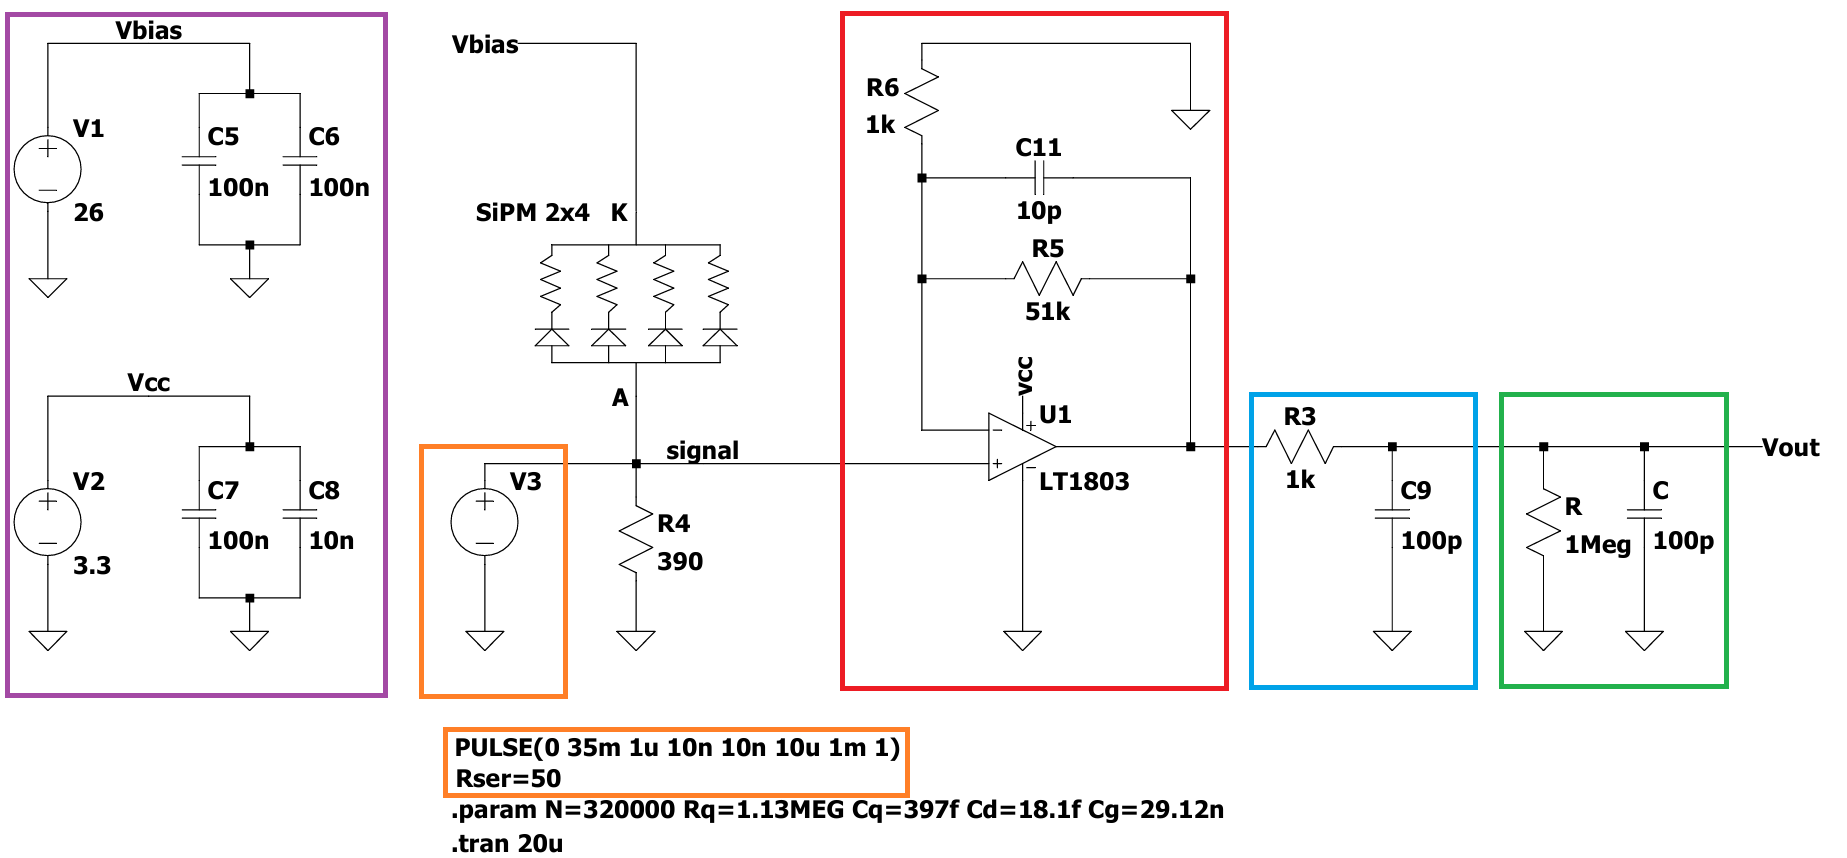
\includegraphics[width=1\textwidth]{voltagemodecircuit_mio.PNG}
		\caption{Circuito schematico nell'ambiente di simulazione LTspice del \gls{sipm} controllato in tensione. In viola l'alimentazione con bypass per filtraggio del rumore. In arancione il segnale di test per la caratterizzazione, in rosso lo stadio di amplificazione, in azzurro un filtro passa-basso del primo ordine e infine in verde la resistenza e la capacità che vede il circuito dall'oscilloscopio. La resistenza R4 converte la corrente dal \gls{sipm} in tensione.}
		\label{fig:scheda_voltagemode_mio}
	\end{figure}
	
	\newpage
	
	Il circuito di condizionamento è un amplificatore non invertente di guadagno:
	\begin{equation}
		Av = 1+\frac{R5}{R6} = 1 + \frac{51K\Omega}{1K\Omega} = 52
	\end{equation}
	in cascata con un filtro passa-basso del primo ordine realizzato da R3 e C9. 
	La caratterizzazione del circuito stampato è stata effettuata con un gradino in ingresso da Vin=35 mV e di ampiezza $5\mu s$, in modo che una volta amplificato:
	\begin{equation}
		Vout = Av \cdot Vin = 52 \cdot 0.035V = 1.82V
	\end{equation}
	l'amplificatore non vada in saturazione dato che non ci si avvicina alla tensione di alimentazione. La misura con gradino applicato esternamente è stata effettuata con e senza \gls{sipm} inserito e con varie tensioni di bias. La caratterizzazione si è estesa anche alla misura con particelle alpha e beta tramite una fenditura di diametro $3mm$ con solamente metà \gls{sipm} connesso, quindi otto celle.
	\begin{figure}[H]
		\centering
		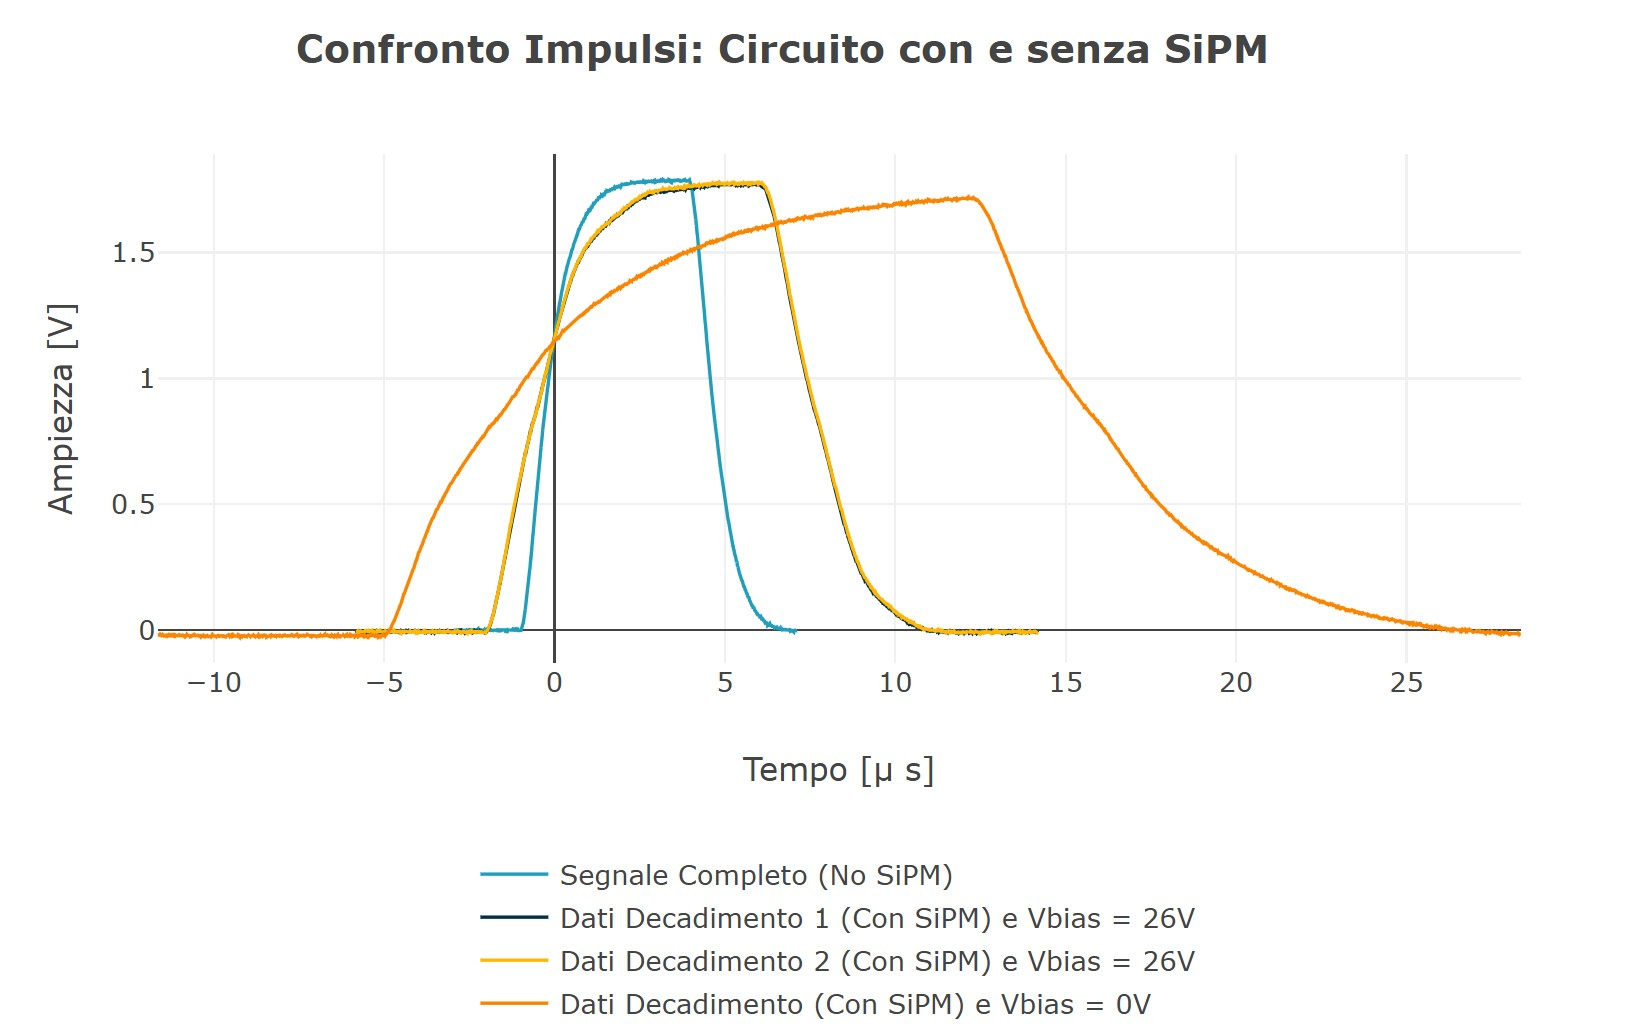
\includegraphics[width=0.85\textwidth]{impulsi_gradino_ext.jpg}
		\label{fig:impulsi_gradino_ext}
		\caption{Quattro diagrammi che mostrano diverse risposte del circuito allo stesso gradino in base alla presenza del \gls{sipm} con diverse tensioni di bias}
	\end{figure}
	\begin{figure}[H]
		\centering
		% Sottofigura di SINISTRA
		\begin{subfigure}[t]{0.48\textwidth} % Cambiato in [t]
			\centering
			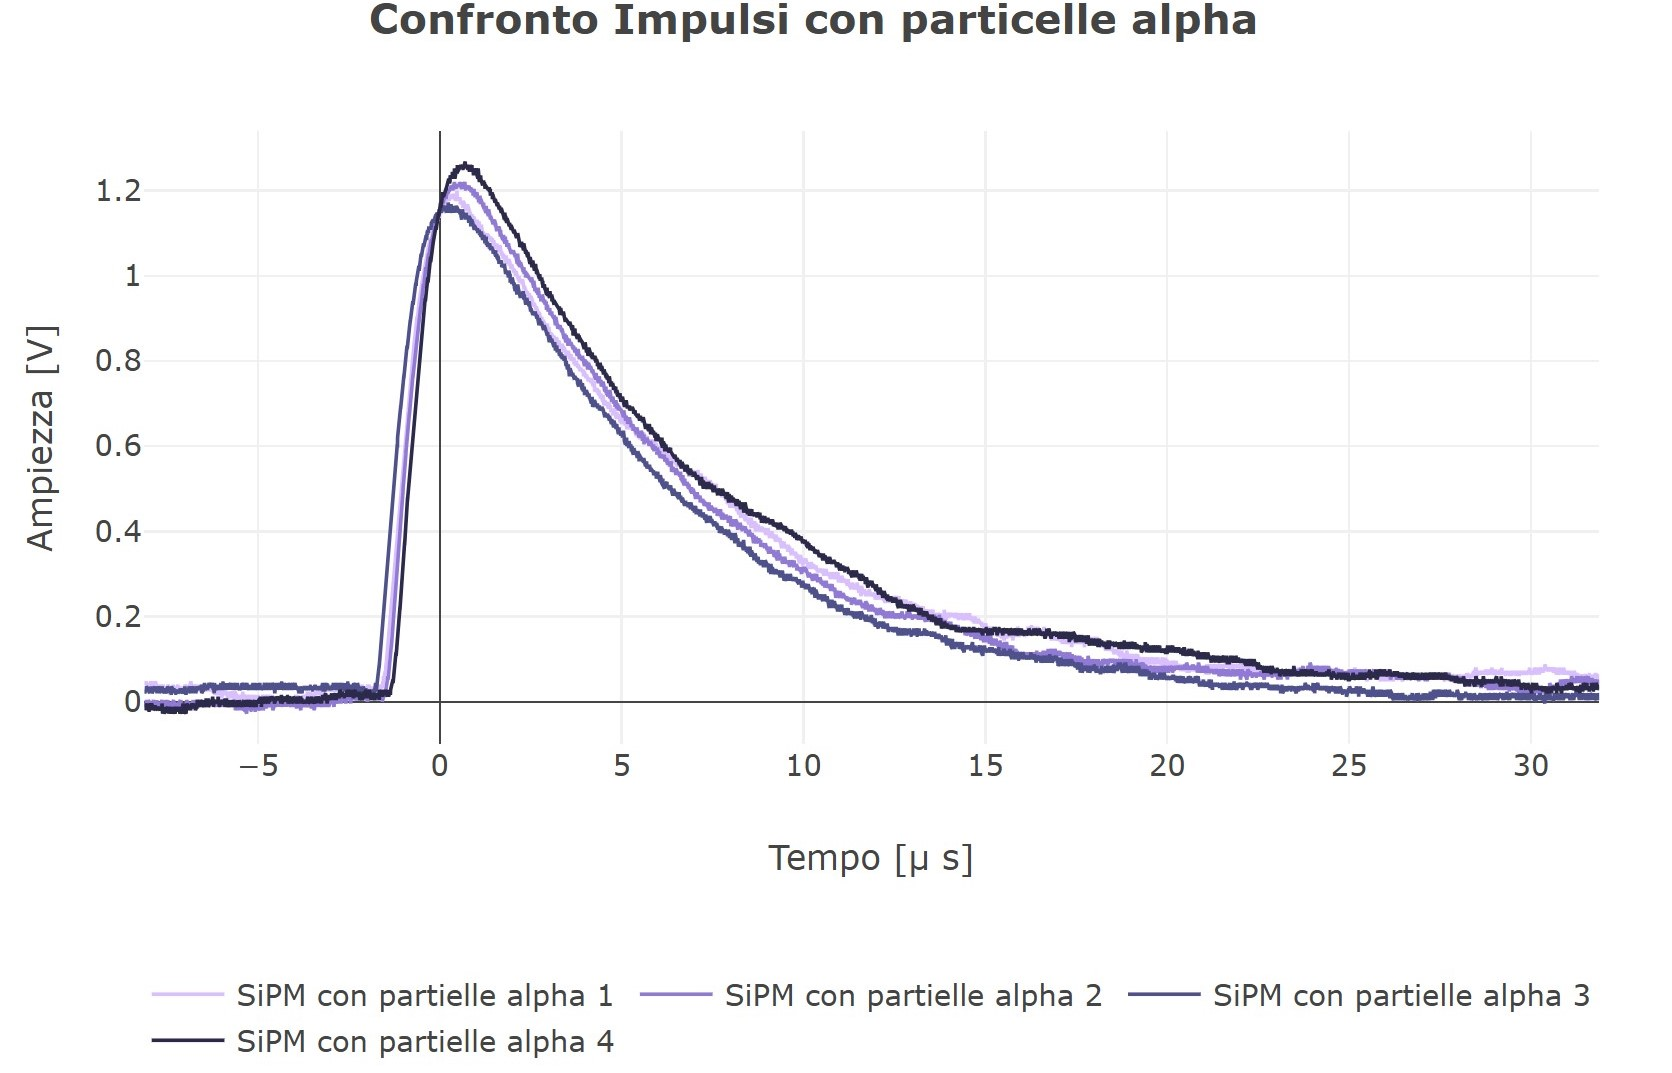
\includegraphics[width=\linewidth]{impulsi_alpha.jpg}
			\caption{Segnale di output della scheda con particelle alpha emesse da un disco di Americio 241 da $3KBq$ e $5.5 MeV$}
			\label{fig:impulsi_alpha}
		\end{subfigure}
		\hfill
		% Sottofigura di DESTRA
		\begin{subfigure}[t]{0.48\textwidth} % Cambiato in [t]
			\centering
			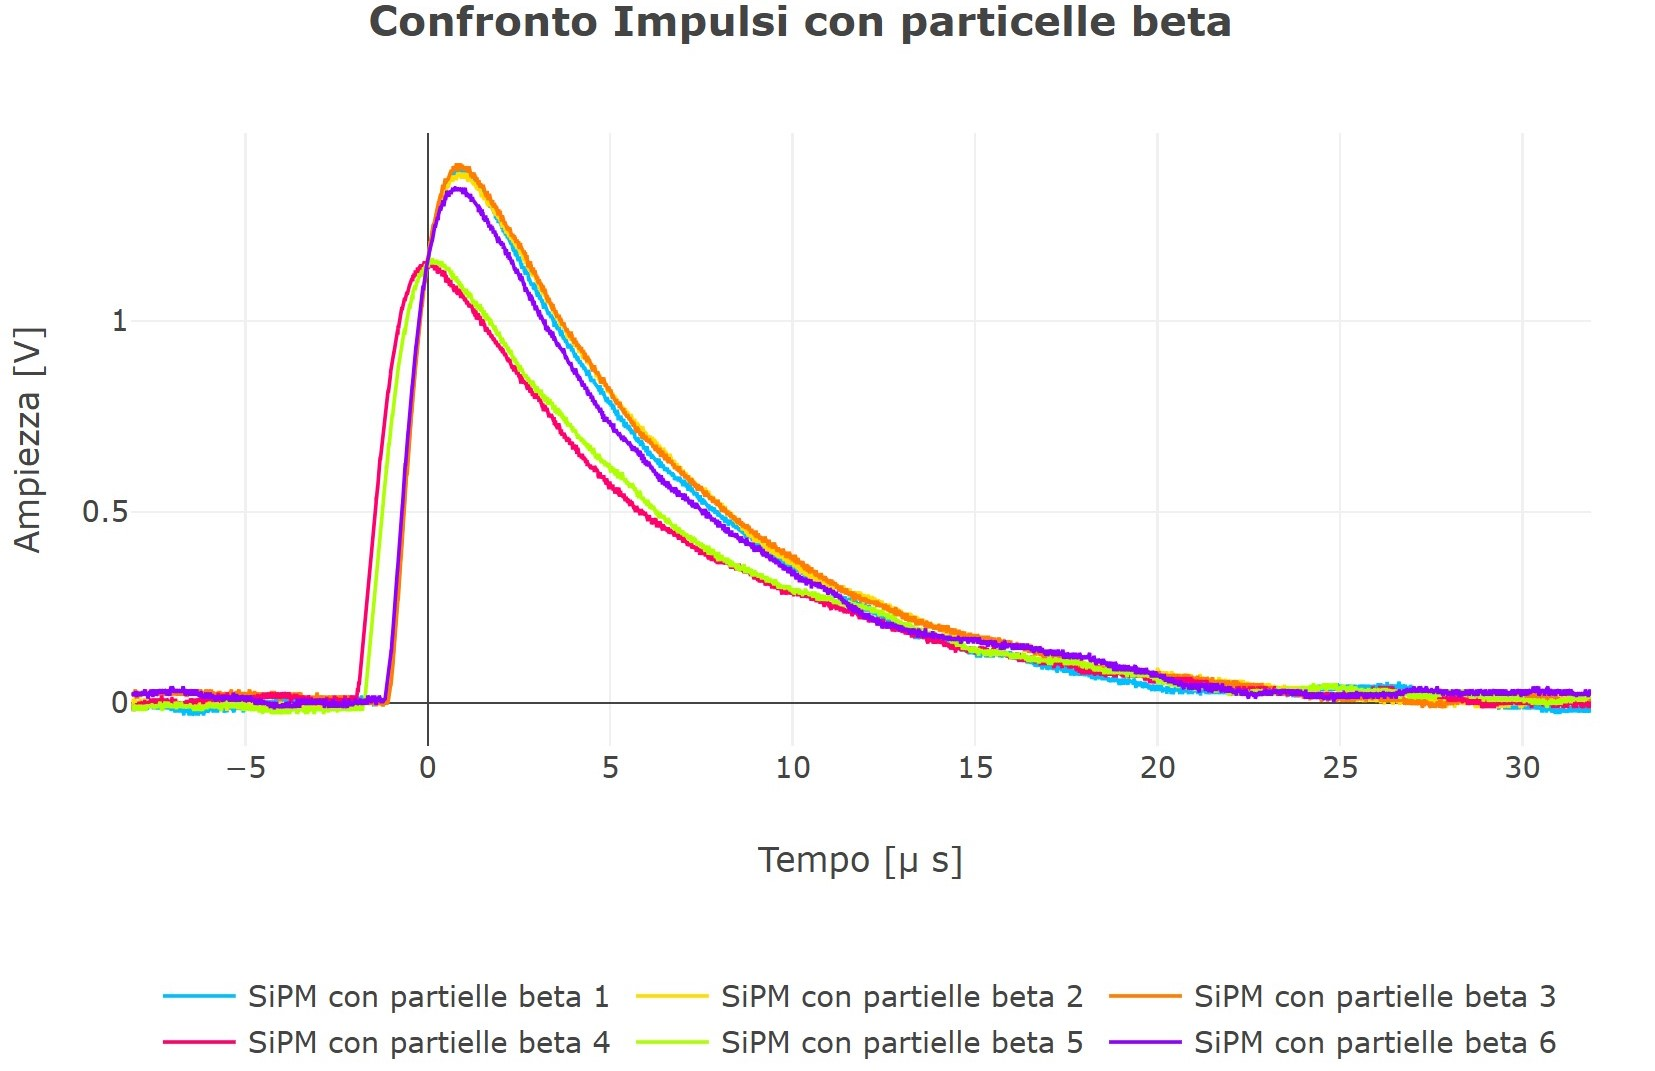
\includegraphics[width=\linewidth]{impulsi_beta.jpg}
			\caption{Segnale di output della scheda con particelle beta emesse da un disco di Stronzio 90 da $18.5KBq$}
			\label{fig:impulsi_beta}
		\end{subfigure}
	\end{figure}
	
	Dopo aver fatto una regressione a singolo e a doppio esponenziale:
	\begin{equation}
		V_{1exp}(t) = A \cdot e^{-\frac{t}{\tau}}+Offset \qquad V_{2exp}(t) = A1 \cdot e^{-\frac{t}{\tau 1}}+A2 \cdot e^{-\frac{t}{\tau 2}}+ Offset
	\end{equation}
	
	per ogni segnale acquisito si procede con il confronto tra la simulazione in LTspice e le misure reali, in modo da essere certi di avere un modello sufficientemente accurato.
	
	\begin{figure}[H]
		\centering
		% Sottofigura di SINISTRA
		\begin{subfigure}[t]{0.48\textwidth} % Cambiato in [t]
			\centering
			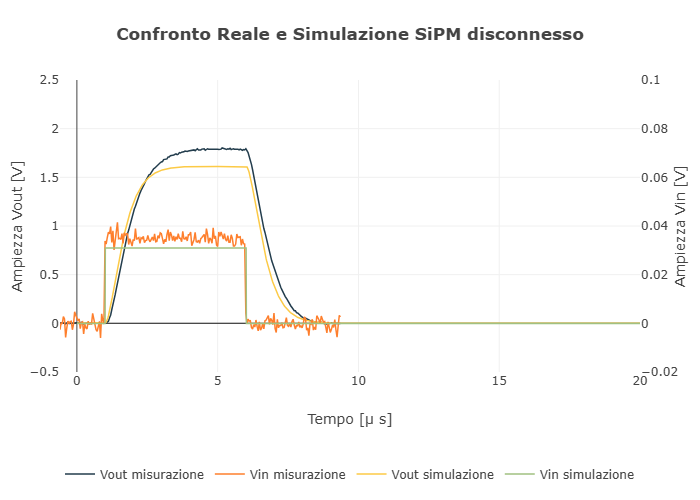
\includegraphics[width=\linewidth]{confronto_no_sipm.png}
			\caption{Segnali di input e output in confronto tra simulazione e misure in controllo tensione con \gls{sipm} scollegato. Il segnale di input è un onda quadra a frequenza $1kHz$ e ampiezza $35mV$}
			\label{fig:confronto_no_sipm}
		\end{subfigure}
		\hfill
		% Sottofigura di DESTRA
		\begin{subfigure}[t]{0.48\textwidth} % Cambiato in [t]
			\centering
			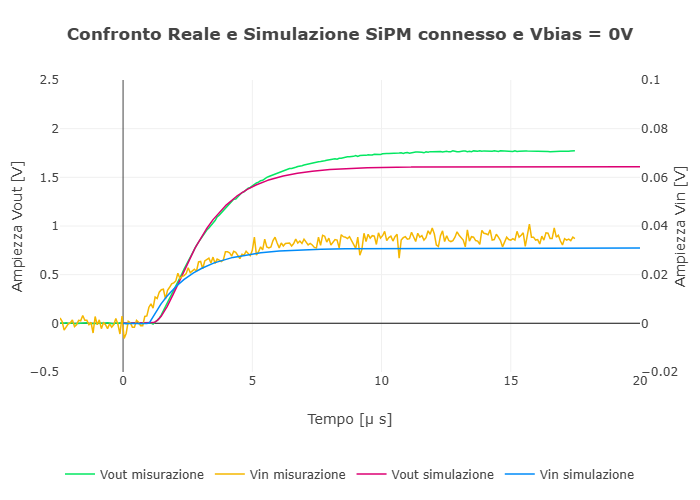
\includegraphics[width=\linewidth]{confronto_sipm_Vbias=0V.png}
			\caption{Segnali di input e output in confronto tra simulazione e misure in controllo tensione con \gls{sipm} alimentato a 0V. Il segnale di input è un impulso di ampiezza $35mV$ e larghezza $5\mu s$}
			\label{fig:confronto_sipm_Vbias=0V}
		\end{subfigure}
	\end{figure}
	\begin{figure}[H]
		\centering
		% Sottofigura di SINISTRA
		\begin{subfigure}[t]{0.48\textwidth} % Cambiato in [t]
			\centering
			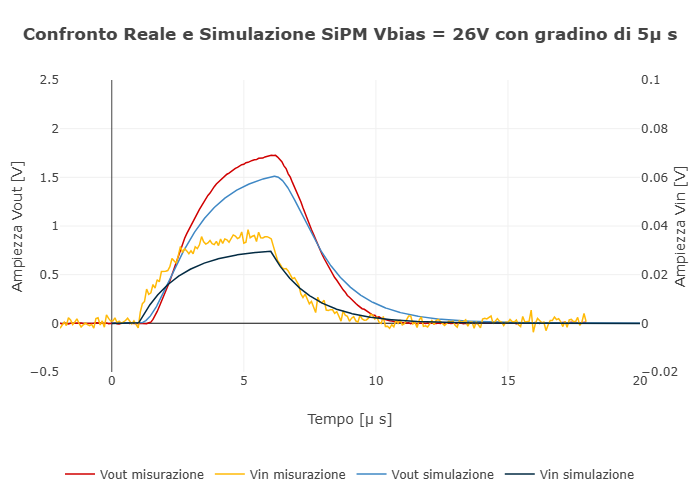
\includegraphics[width=\linewidth]{confronto_sipm_Vbias=26V_5us.png}
			\caption{Segnali di input e output in confronto tra simulazione e misure in controllo tensione con \gls{sipm} alimentato a 26V. Il segnale di input è un impulso di ampiezza $35mV$ e larghezza $5\mu s$}
			\label{fig:confronto_sipm_Vbias=26V_5us}
		\end{subfigure}
		\hfill
		% Sottofigura di DESTRA
		\begin{subfigure}[t]{0.48\textwidth} % Cambiato in [t]
			\centering
			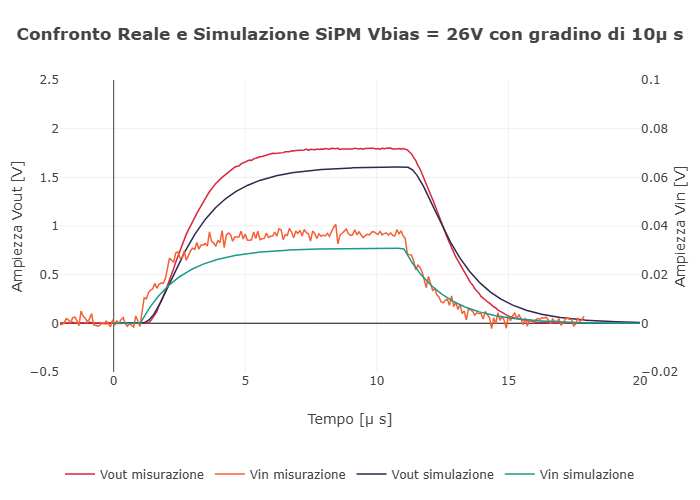
\includegraphics[width=\linewidth]{confronto_sipm_Vbias=26V_10us.png}
			\caption{Segnali di input e output in confronto tra simulazione e misure in controllo tensione con \gls{sipm} alimentato a 26V. Il segnale di input è un impulso di ampiezza $35mV$ e larghezza $10\mu s$}
			\label{fig:confronto_sipm_Vbias=26V_10us}
		\end{subfigure}
	\end{figure}
	
	La valutazione sperimentale e le simulazioni ai piccoli segnali hanno evidenziato limitazioni intrinseche della topologia \textit{voltage-mode} nell'interfacciamento di \gls{sipm} di grande area.
	
	Il limite principale risiede nel \textbf{prodotto guadagno-banda} (\gls{gbw}) dell'amplificatore operazionale, che vincola fortemente la larghezza di banda a ciclo chiuso. Questo fenomeno sopprime le componenti ad alta frequenza dell'impulso a valanga del \gls{sipm}, producendo un segnale di uscita marcatamente più lento.
	\newpage
	L'analisi evidenzia un compromesso critico legato alla resistenza di \textit{shunt} (Nello schema di \textbf{Fig:\ref{fig:scheda_voltagemode_mio}} corrisponde alla R4 di $390\Omega$) utilizzata per la conversione corrente-tensione:
	\begin{itemize}
		\item Una resistenza di \textit{shunt} ridotta velocizzerebbe il segnale, rendendo la caduta di tensione meno sensibile ai transienti rapidi.
		\item Tuttatavia, la riduzione della resistenza diminuisce proporzionalmente l'ampiezza in uscita, costringendo lo stadio di amplificazione successivo a fornire un guadagno maggiore.
		\item L'aumento del guadagno esaspera ulteriormente il limite del \gls{gbw}, riducendo la banda effettaiva e aumentando la distorsione dell'impulso rapido del sensore.
	\end{itemize}
	
	A patto di un fattore di offset dovuto alla tolleranza delle resistenze il modello simulato si comporta come nella realtà. Ma in conclusione, i vincoli descritti precedentemente impediscono alla configurazione in tensione di riprodurre fedelmente i segnali veloci tipici dei \gls{sipm}.
	
	\subsection{Controllo in Corrente}
	La lettura in corrente può essere implementata con un \gls{tia}
	\begin{figure}[H]
		\centering
		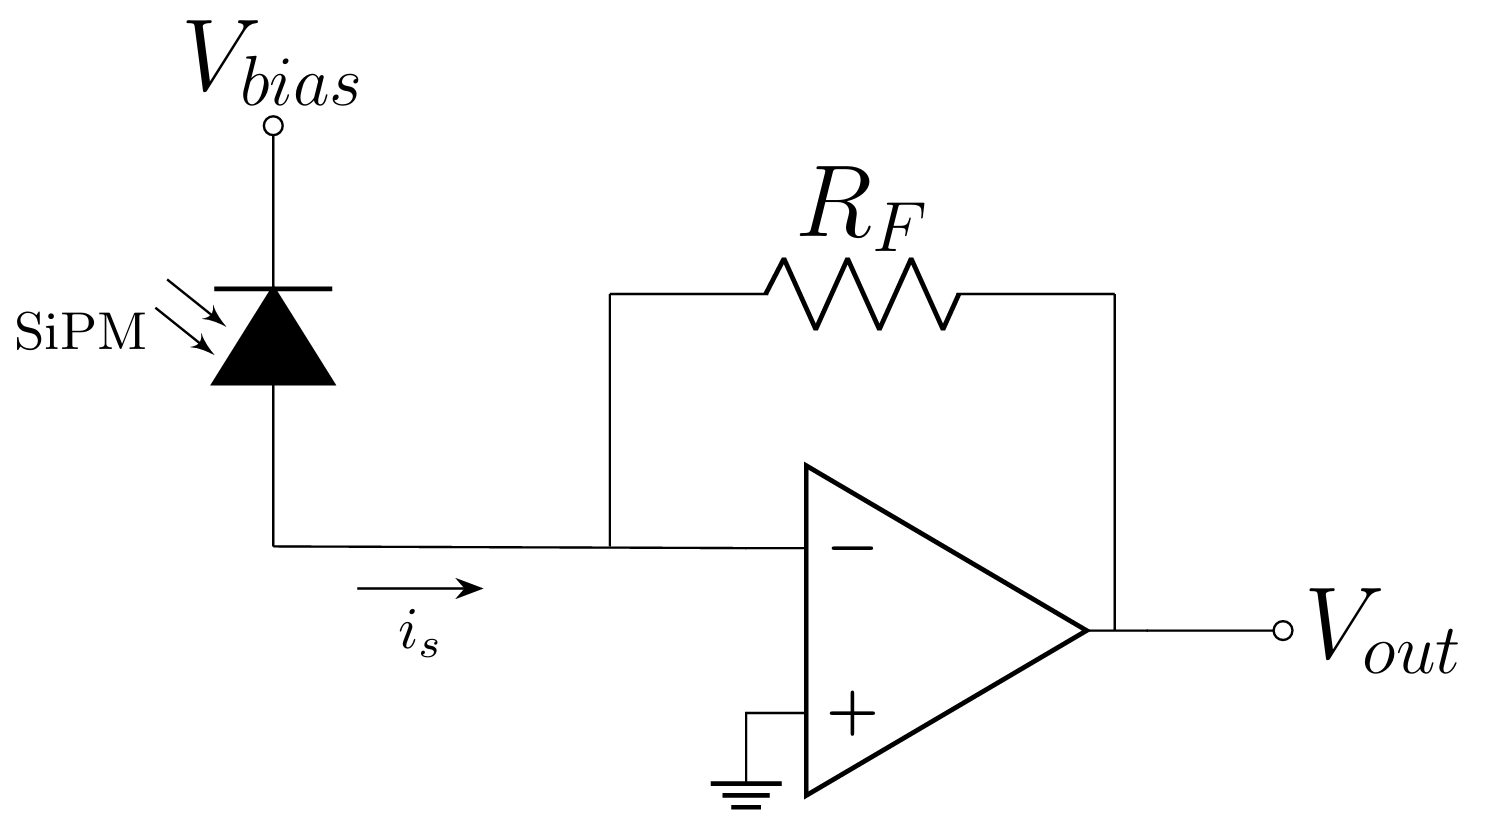
\includegraphics[width=0.5\textwidth]{tia.PNG}
		\caption{Amplificatore in corrente con \gls{tia}}
		\label{fig:tia}
	\end{figure}
	
	L'espressione di $Vout$ è:
	\begin{equation}
		\centering
		V_{out} = -RF \cdot i_s
	\end{equation}
	
	L'obiettivo di questo circuito rispetto al controllo in tensione è di aumentare la velocità del segnale in uscita, in modo da avere una finestra temporale più ampia per ridurre il più possibile il fenomeno di pile up. Convertendo la corrente all'interno dell'anello di retroazione, rispetto con la resistenza di \textit{shunt}, si avrà una risposta più veloce.
	
	Il circuito di condizionamento per la lettura in corrente è composto da due stadi, il primo è il \gls{tia}, per la conversione corrente-tensione mentre il secondo stadio è un amplificatore differenziale, per regolare il fondo scala e l'amplificazione adeguata per una lettura al massimo delle potenzialità del HW. 
	
	\begin{equation}
		V+ = VCC \cdot  \frac{R}{R+R} = \frac{VCC}{2}
	\end{equation}
	
	\begin{figure}[H]
		\centering
		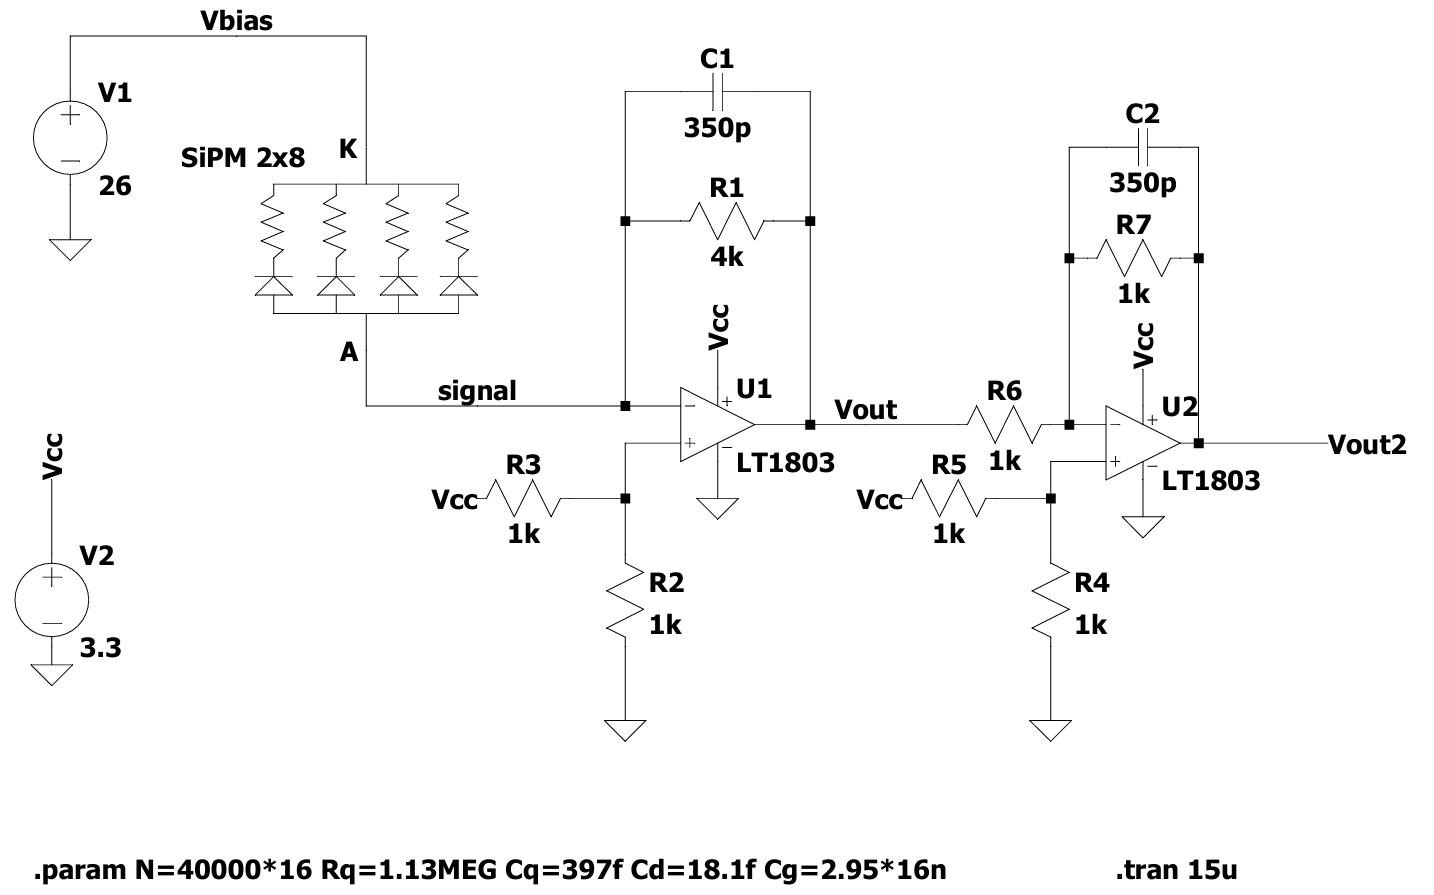
\includegraphics[width=1\textwidth]{mio_circuito_controllo_corrente.PNG}
		\caption{Circuito \gls{sipm} controllato in corrente}
		\label{fig:mio_circuito_controllo_corrente}
	\end{figure}
	
	La tensione di alimentazione(VCC)per gli \gls{opamp} va da 0 a 3.3V. Le resistenze uguali al morsetto positivo formano un partitore di tensione e hanno la funzionalità di impostare il segnale di base a VCC/2, in modo da avere uno spettro più ampio di tensione del segnale, dato che l'uscita del \gls{tia} altrimenti dovrebbe avere valori negativi, ma l'alimentazione è strettamente positiva.
	
	L'amplificatore differenziale ha il solo scopo di invertire il segnale in uscita dal primo stadio, dato il suo guadagno:
	\begin{equation}
		Av = \frac{R7}{R4} = \frac{10^3}{10^3} = 1
	\end{equation}
	
	Infine gli amplificatori C1 e C2 sono dimensionati per evitare il sottosmorzamento del sistema cercando di avere i poli reali e più vicini possibile.

	Lo stesso impulso uscente dal generatore di corrente del modello equivalente del SiPM, impostato per dare un'ampiezza pari a quella delle particelle alpha misurato in laboratorio, confrontato tra i due modelli circuitali sia con 8 che 16 celle connese al \gls{sipm}
	
	\begin{figure}[H]
		\centering
		
\includegraphics[width=0.9\textwidth]{confronto_currentmode_voltagemode_8_SiPM.png}
		\caption{Confronto con lo stesso segnale uscente dalle 8 celle del \gls{sipm} tra circuito controllato in tensione (vout = linea rossa) e il circuito controllato in corrente (vout2 = blu)}
		\label{fig:confronto_currentmode_voltagemode_8_SiPM}
	\end{figure}
	
	\begin{figure}[H]
		\centering
		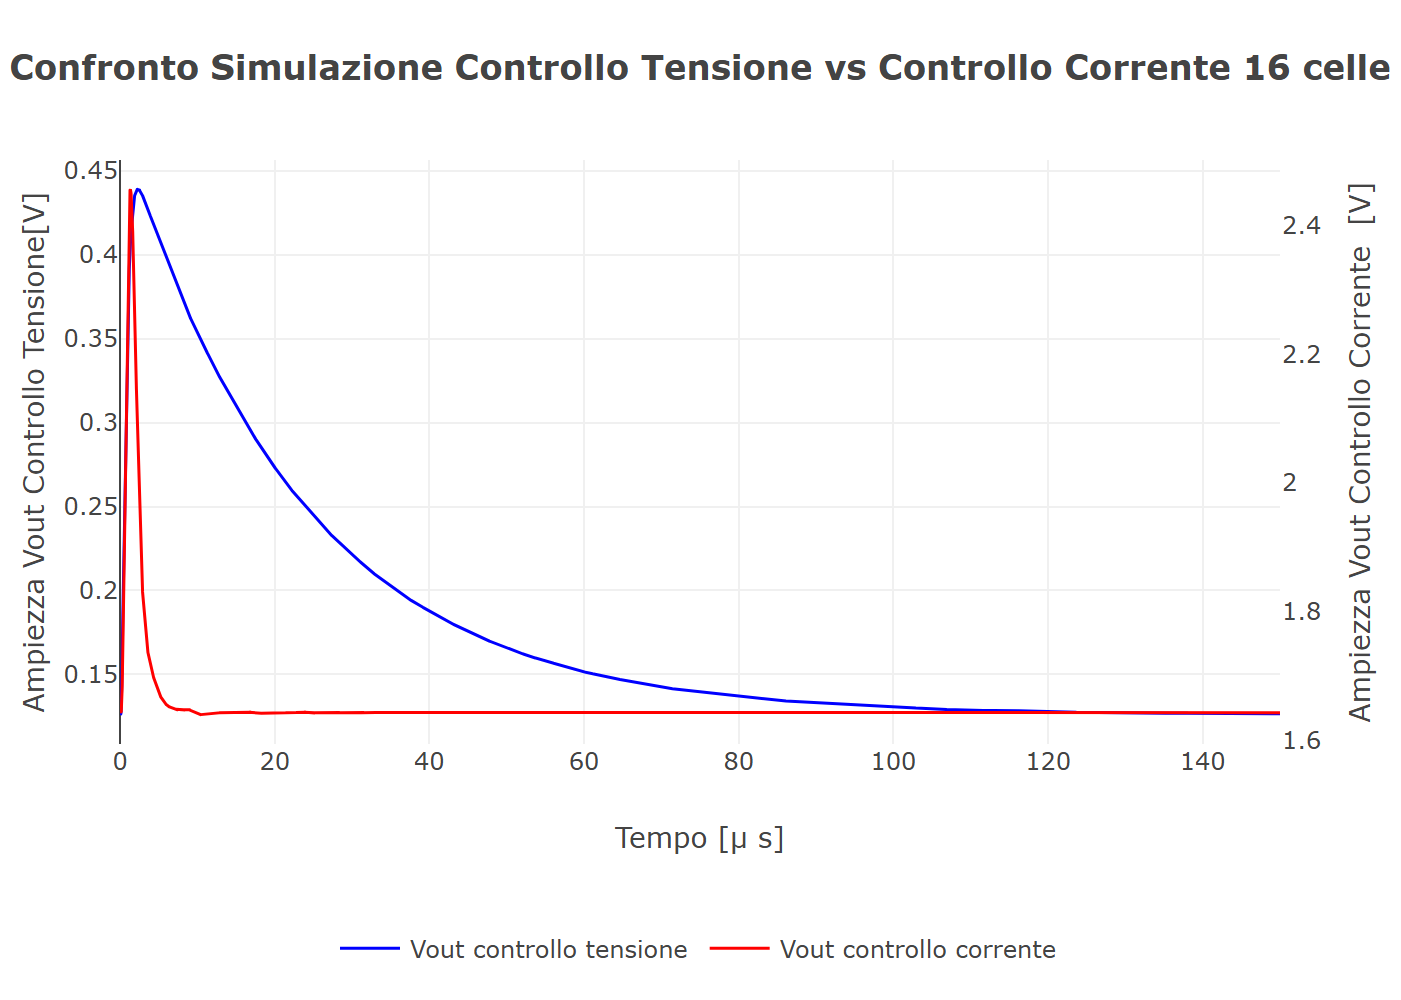
\includegraphics[width=0.9\textwidth]{confronto_currentmode_voltagemode_16_SiPM.png}
		\caption{Confronto con lo stesso segnale uscente dalle 16 celle del \gls{sipm} tra circuito controllato in tensione (vout = linea rossa) e il circuito controllato in corrente (vout2 = blu)}
		\label{fig:confronto_currentmode_voltagemode_16_SiPM}
	\end{figure}
	
	\begin{table}[H]
		\centering
		% Prima tabella (Sinistra)
		\begin{minipage}{0.48\textwidth}
			\centering
			\begin{tabular}{l|c|r}
				\hline
				Tempo & 8 celle & 16 celle \\ \hline
				Trise [$\mu s$]&  0.99551 & 1.07831 \\ 
				Tfall [$\mu s$]&  25.22879 & 50.23618 \\ 
			\end{tabular}
			\caption{{\small Tempi Controllo Tensione}}
		\end{minipage}
		\hfill % Spazio elastico centrale
		% Seconda tabella (Destra)
		\begin{minipage}{0.48\textwidth}
			\centering
			\begin{tabular}{l|c|r}
				\hline
				Tempo & 8 celle & 16 celle \\ \hline
				Trise [$\mu s$] &  0.51812 & 0.71022 \\ 
				Tfall [$\mu s$]&  2.74100 & 2.16989 \\ 
			\end{tabular}
			\caption{{\small Tempi Controllo Corrente}}
		\end{minipage}
	\end{table}
	

	%bibliografia 
	\newpage
	\printbibliography
\end{document}